\chapter{Executive Summary}
\label{ch:exec-overall}

%%%%%%%%%%%%%%%%%%%%%%%%%%%%%%%%%%%%%%%%%%%%%%%%%%%%%%%%%%%
\section{Overview}
\label{sec:exec-overall-1}

%%%%%%%%%%%%%%%%%%%%%%%%%%%%%%
\subsection{The DUNE Science Program, Detectors, and Supporting Facilities}

The international \dword{dune} will be a world-class neutrino observatory and nucleon decay detector designed to answer fundamental questions about elementary particles and their role in the universe. The experiment will carry out a comprehensive program of neutrino oscillation measurements, aiming for the discovery of \dword{cpv} in neutrino oscillations, which may give insight into the origin of the matter-antimatter asymmetry in the  universe. 
\dword{dune} will also 
detect and measure the electron neutrino ($\nu_\text{e}$) flux from a core-collapse supernova within the Milky Way, should one occur during the lifetime of the experiment. Such a measurement would provide a wealth of unique information about the early stages of core collapse and could signal the birth of a black hole. The experiment's third primary goal is a search for proton decay in several decay modes and for other baryon-number-violating processes. The observation of baryon number violation would represent a ground-breaking discovery in physics, providing a key requirement for grand unification of the forces.

The international experiment, hosted by the U.S. Department of Energy's \dword{fnal}, will consist of a \dword{fd} located approximately \SI{1.5}{km} underground at the \dword{surf} in South Dakota, USA, \SI{1300}{\km} from \dword{fnal}, and a %multi-functional 
\dword{nd} located at \dword{fnal} in Illinois (Figure~\ref{fig:lbnf}). The far detector, the subject of this \dword{tdr}, will be a very large, modular \dword{lartpc} with a \fdfiducialmass (\SI{40}{\giga\gram}\footnote{This is nearly the mass of a standard fast battleship, for comparison.}) %fiducial 
target mass of \dword{lar} that  
can uniquely reconstruct neutrino interactions with image-like precision and unprecedented resolution. 

\begin{dunefigure}[ 	
Configuration of the LBNF beam and the DUNE detectors]{fig:lbnf}{ 	
Cartoon illustrating the configuration of the LBNF beamline at Fermilab, in Illinois, and the DUNE detectors in Illinois and South Dakota, separated by \SI{1300}{km}.}
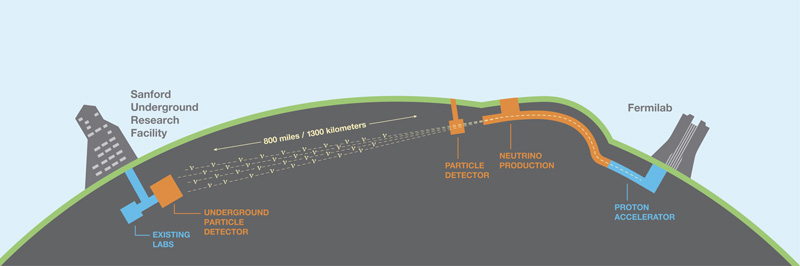
\includegraphics[width=0.9\textwidth]{lbnf_dune_graphic_miles_km-15-0031-01.jpg}
\end{dunefigure}


                                       %%% try moving LBNF stuff here %%%%%
The \dword{lbnf} project, also hosted by \dword{fnal}, provides the beamline and the civil construction, called \dword{cf}, for the \dword{dune} experiment.  %this complex system of detectors at the Illinois and South Dakota sites. 
The organization and management of \dword{lbnf} is separate from that of the experiment; its design and construction are organized as a U.S. \dword{doe}/\dword{fnal} project incorporating international partners. 

The \dword{lbnf} %is responsible for building a 
beamline at \dword{fnal} will deliver the world's most intense neutrino beam to the near and far detectors in an on-axis configuration. %This project will also prepare the housing and infrastructure for the detectors, including excavation and outfitting of three deep-underground caverns for the \dword{fd}. 
%The U.S. DOE \dword{lbnf} project 
%The project is building a facility at \dword{surf} that will house and provide infrastructure for the first two \dword{dune} \dword{fd} modules and another at \dword{fnal} for the \dword{nd}.  
%At the start of \dword{dune} operations \dword{pip2}, will deliver protons in the energy range \SIrange{60}{120}{\GeV}. 
The upgrade to the  \dword{pip2}~\cite{pip2-2013}, a leading-edge, superconducting, linear proton accelerator under construction at \dword{fnal}~\cite{pip2-2013}, will deliver between \num{1.0} and \SI{1.2}{MW} of proton beam power from the \dword{fnal} Main Injector to \dword{lbnf}, which will aim and focus the beam, whereupon the protons,  in the energy range \SIrange{60}{120}{\GeV}, will collide with a target, creating a secondary beam from which the intense neutrino flux will emerge, traveling in the direction of the \dword{dune} detectors (Figure~\ref{fig:beamline}).   A further planned upgrade 
of the accelerator complex could provide up to \SI{2.4}{\MW} of beam power by 2030, 
%The continuous-wave-compatible, modern superconducting radio-frequency linac of \dword{pip2} will provide a platform for extending beam power for \dword{dune} to multi-\si{MW} capability, 
potentially extending the \dword{dune} science reach. The upgrade will also increase the reliability of the \dword{fnal} accelerator complex and provide the flexibility to produce customized  beams tailored to specific scientific needs.

\begin{dunefigure}[Neutrino beamline and DUNE near detector hall in Illinois
]{fig:beamline}{Neutrino beamline and \dword{dune}{} near detector hall at \dword{fnal}{} in Illinois}
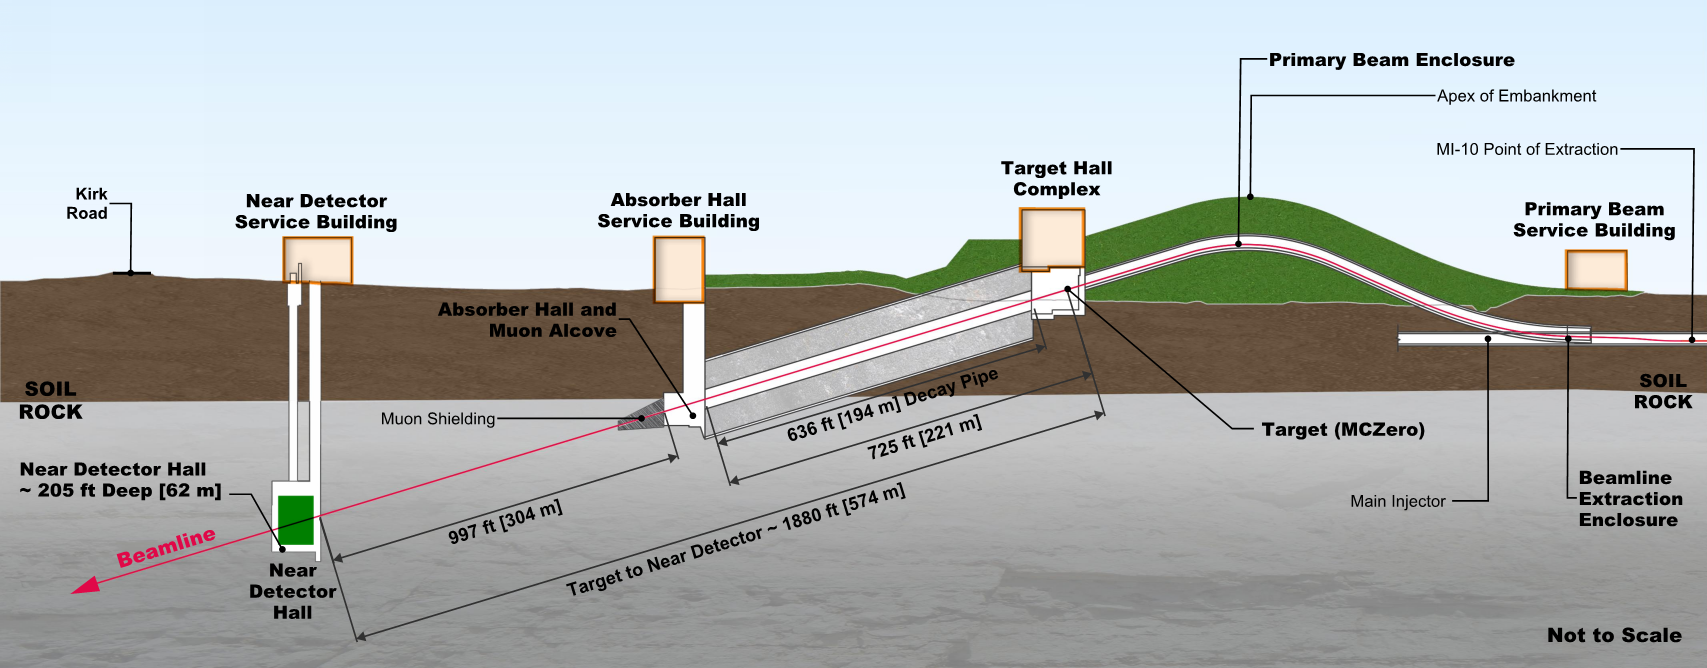
\includegraphics[width=0.9\textwidth]{beamline-sideview.jpg}
\end{dunefigure}

The intense, wide-band neutrino beam, the massive \dword{lartpc} detector at the far site, and the high-resolution
\dword{nd} will provide a rich ancillary science program for the \dword{dune} experiment, beyond its primary goals,   
including accelerator-based neutrino flavor-transition measurements with sensitivity to physics beyond the standard model, measurements of tau neutrino appearance, measurements of neutrino oscillation phenomena using atmospheric neutrinos, and  a rich neutrino interaction physics program using the \dword{dune} \dword{nd}, including a wide range of measurements of neutrino cross sections and studies of nuclear effects, and searches for dark matter. 
\fixme{is DM search only available w ND?}
Further advances in \dword{lartpc} 
technology during  \dword{fd} construction may open up possibilities to observe very low-energy phenomena such as solar neutrinos or even the diffuse supernova neutrino flux -- measurements that require a sensitivity that is presently beyond our reach.

%%%%%%%%%%%%%%%%%%%%%%%%%%%%%%
\subsection{The DUNE Collaboration}

The \dword{dune} collaboration is a global organization with more than \num{1000} scientists and engineers from \num{31} countries (Figure~\ref{fig:map2}). It represents the combination of several worldwide efforts that developed independent paths toward a next-generation long-baseline neutrino experiment over the last decade. \dword{dune} was formed in April 2015, combining the strengths of the \dword{lbne} project in the U.S. and the \dword{lbno} project in Europe, adding many new international partners in the process. \dword{dune} thus represents the convergence of a substantial fraction of the worldwide neutrino-physics community around the opportunity provided by the large investment planned by the U.S. \dword{doe} and \dword{fnal} to support a significant expansion of the underground infrastructure at \dword{surf} in South Dakota and to create a megawatt neutrino-beam facility at \dword{fnal}. 

\begin{dunefigure}[DUNE collaboration global map]{fig:map2}{The international \dword{dune}
collaboration. Countries with \dword{dune} membership are in orange.}
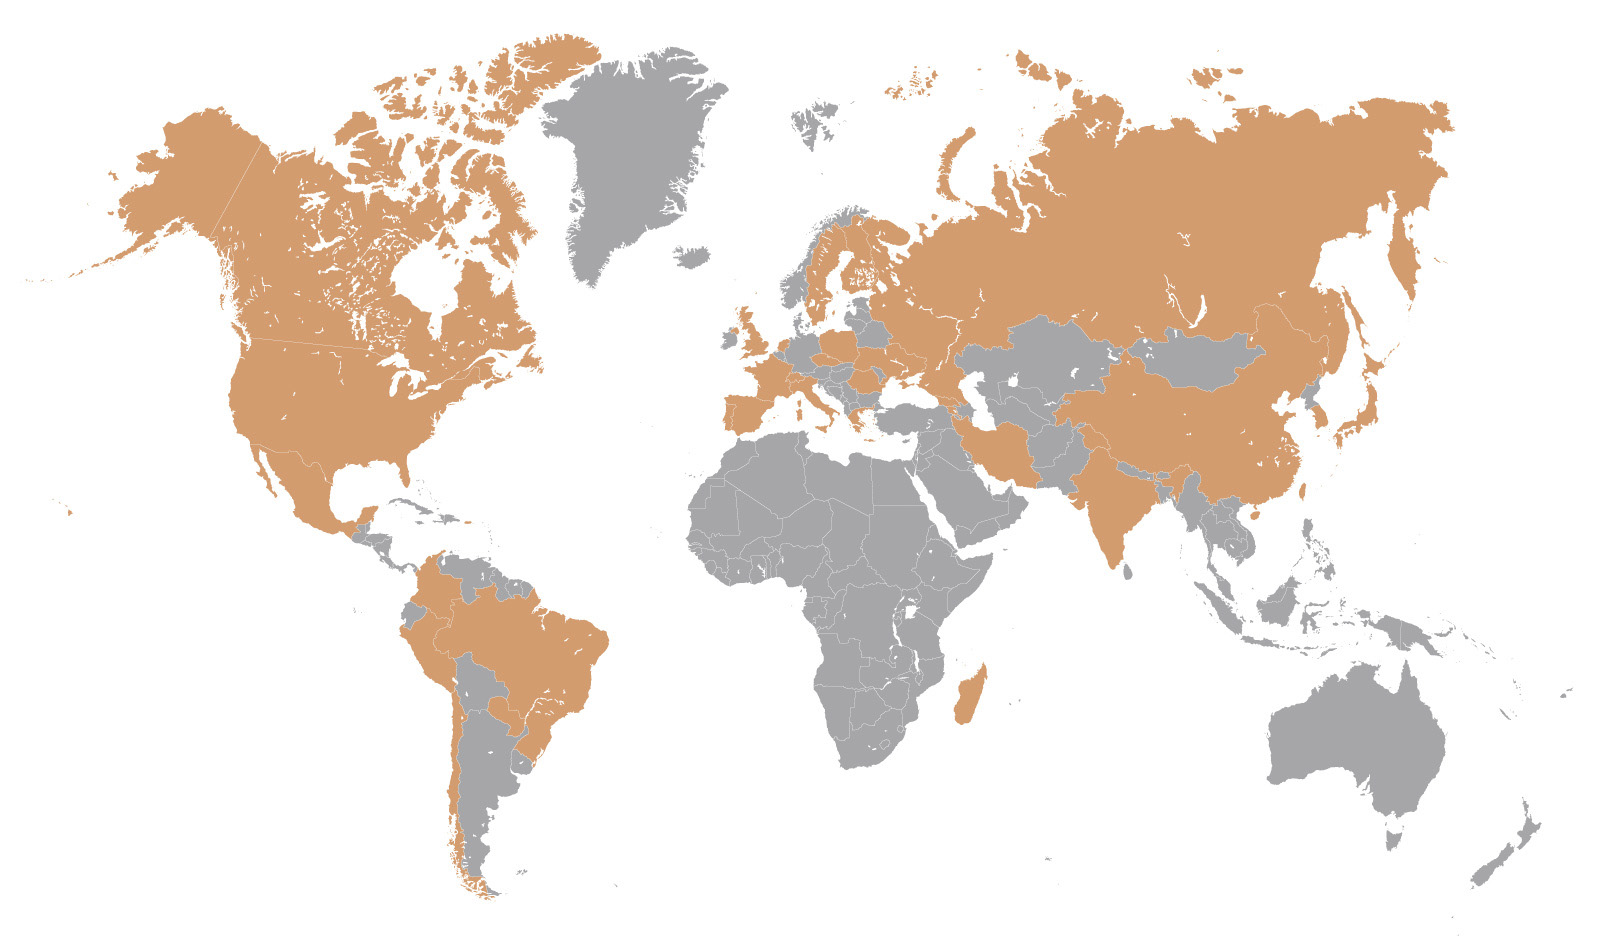
\includegraphics[width=0.9\textwidth]{dune-countries-july2019.jpg}  
\end{dunefigure} %updated by anne 7/15

%%%%%%%%%%%%%%%%%%%%%%%%%%%%%%%%
\subsection{Strategy for the DUNE Far Detector Design}

% start from SB IPR talk
%The \dword{lbnf}/\dword{dune} strategy presented in this \dword{tdr} has been developed to meet the requirements laid
\dword{dune} and \dword{lbnf} have developed the strategy presented in this \dword{tdr} to meet the requirements laid 
out in the report of the U.S. Particle Physics Project Prioritization Panel (P5) in 2014. The strategy also takes into account the recommendations of the \dword{espp} adopted by the \dword{cern} Council in 2013, which classified the long-baseline neutrino program as one of the four scientific objectives requiring significant resources, sizable collaborations, and sustained commitment.

The P5 report~\cite{p5report} set the goal of reaching a sensitivity to \dword{cpv} of more than three standard deviations (\num{3}$\sigma$) over more than $75\%$ 
of the range of possible values of the unknown \dshort{cp}-violating phase \deltacp.
 Based partly on this goal, the report stated that ``the 
minimum requirements to proceed are the identified capability to reach an exposure 
of \num{120}~\ktMWyr{} by the 2035 time frame, the far detector situated underground 
with cavern space for expansion to at least \fdfiducialmass \dword{lar} fiducial volume, and \SI{1.2}{MW} beam power upgradeable to multi-megawatt power.
The experiment should have the demonstrated 
capability to search for \dwords{snb} and for proton decay, providing a significant 
improvement in discovery sensitivity over current searches for proton decay.'' %The strategy and design presented in this \dword{tdr} meet these requirements.


Here we briefly address how the \dword{lbnf-dune} strategy and designs will satisfiy each of these requirements and deliver a world-leading neutrino program. %These concepts are further described in 
The following chapters and the other volumes of this \dword{tdr} elaborate on these concepts, providing a full picture of this ambitious enterprise. 

\textit{Reach at least \SI{120}{\msr} exposure by the 2035 timeframe and \SI{1.2}{\MW} beam power: } To reach the necessary precision on its measurements, \dword{dune} will need to collect a few thousand neutrino interactions over a period of about ten years. The number of interactions is the product of (1) the intensity of the neutrino beam, (2) the probability that a neutrino will oscillate (approximately \num{0.02}), (3) the interaction cross section, and (4) the detector mass.  Currently, the highest-power proton beam that a beam target can safely withstand is between \num{1} and \SI{2}{\MW}, which caps the achievable neutrino beam intensity. This points to a required a detector mass in the tens-of-kilotons range. The \dword{dune} \dword{fd} is designed to be \fdfiducialmass{}.

%from phys chapter (prev 2.2):
Moreover, the \dword{dune} concept
    builds on the notion that a highly-performant detector technology  
    with excellent neutrino energy reconstruction
    and background rejection capabilities can
    optimize sensitivity and cost with an on-axis exposure to
    an intense, wide-band, conventional (magnetic horn-focused) beam.
   The current generation of long-baseline neutrino experiments
	have benefited from narrow-band beam characteristics 
	associated with off-axis detector deployment, which offers 
	a low background rate in both \nue appearance 
	and \numu disappearance channels. % from misidentified \dword{nc}  interactions of high energy neutrinos.  
	However, this advantage comes at a cost of flux and 
	spectral information relative to an on-axis detector 
    configuration~\cite{Adams:2013qkq,Agarwalla:2014tca}.
    

\textit{Situated underground:}
Given the rate of cosmic rays at the surface (\SI{165}{kHz}) and the neutrino beam parameters, the ratio of neutrino events to cosmic rays would be less than one to a million and the discovery potential for \dword{dune}'s oscillation physics goals would be vanishingly small.  Roughly \SI{1500}{m} underground at the \dword{surf} site, this ratio becomes slightly higher than 1, raising the potential to a very achievable level.  Supernova neutrinos have energies on the order of \num{100} times lower than beam neutrinos, and despite the fact that they arrive in a few-second burst, would be nearly impossible to identify on the surface. A meaningful search for nucleon decay is not possible at the surface. All three of the experiment's primary goals require significant overburden for the \dword{fd}, which the \dword{surf} site provides. 

\textit{Use of \dword{lar}:}
This requirement implies the use of \dword{lartpc} technology, which enables finer resolution for kiloton-scale particle
detectors than earlier technologies do. The enhanced resolution leads to greater efficiency in distinguishing signal events from background, which in turn leads to a reduction in the necessary size of the detector and potentially broadens the physics program.
%from phys chapter (prev 2.2):
    It is especially important for the long-baseline program with the  
    wide-band neutrino beam.
    Additionally, the choice of \dword{lartpc} technology provides 
    valuable complementarity to other 
    existing and planned detectors pursuing many
    of the same goals.  As an example,
    the sensitivity of \dword{dune} to the \nue component of supernova 
    neutrino flux, prevalent in the neutronization phase of the 
    explosion, provides distinct information relative to that 
    provided by water or organic scintillator-based detectors in 
    which \anue interactions dominate. 

\textit{Sensitivity to \dword{cpv}:}
The physics that \dword{dune} will pursue demands measurements at the few-percent level. With just a \dword{fd}, the neutrino fluxes would be known only to about \SI{10}{\%} and interaction rates to at best \SI{20}{\%}.  To adequately reduce the uncertainties, is necessary to measure the neutrinos at a near location, e.g., \SI{500}{m} from the neutrino source and  at a far location, e.g., \SI{1300}{km} away, using the same target nucleus in both detectors, and to extract the physics measurements from differences between the two.  The \dword{nd} can be smaller than the \dword{fd}, but it must be multi-functional since the differences in the measurements are not due solely to the oscillations.  The detector rate is the product of the neutrino flux, the detector response, and the interaction cross section, the first two of which will differ between the \dword{nd} and \dword{fd} due to other factors as well, e.g.,  event rate and geometry. The \dword{nd} must be able to measure the factors that go into the detector rate separately.  

The optimal \dword{fd} distance (baseline) to determine the \dword{mh}, observe \dword{cpv}, and observe \deltacp is between \num{1000} and \SI{2000}{km}; at shorter baselines the optimal neutrino energy is lower, the second oscillation maximum is too low in energy to be visible, and \dword{cp} sensitivity is reduced by ambiguities from the unknown mass ordering. At longer baselines \dword{cp} sensitivity is harmed by matter effects that increase with baseline length. The \SI{1300}{km} baseline offered by locating the \dword{fd} at \dword{surf} is optimized for the neutrino oscillation physics goals of the \dword{dune} program.

% end from SB IPR talk
 % from phys 2.2
 The scientific basis for \dword{dune}'s foundational experimental
design choices has been examined and validated through extensive
review, undertaken at all stages of \dword{dune} development.
Recent experimental and theoretical developments have only
strengthened the scientific case for \dword{dune} and its
basic configuration.  The technical underpinnings for
these choices have also been strengthened over time through a worldwide
program of R\&D and engineering development, as described in a suite
of \dword{lbnf-dune} project documents including this \dword{tdr}, as
well as in sources describing independent experiments and development
activities.

%%%%%%%%%%%%%%%%%%%%%%%%%%%%%%%%%%%%%%%%%%%%%%%%%%%%%%%%%%%%%%%
\section{The Long-Baseline Neutrino Facility (LBNF)} 
\label{sec:exec:lbnf}

As mentioned above, the \dword{lbnf} project will provide the beamline and the \dword{cf} for both detectors of the \dword{dune} experiment. At the far site, \dword{surf} in South Dakota, \dword{lbnf} will construct a facility to house and provide infrastructure for the first two \dword{dune}  \nominalmodsize fiducial mass \dword{fd} modules; in particular \dword{lbnf} is responsible for:

\begin{itemize}
%\item  the  technical and conventional facilities for a powerful neutrino beam using the \dword{pip2} upgrade of the \dword{fnal} accelerator complex; 

%\item  the  \dword{cf} for the \dword{nd} systems at \dword{fnal} (Figure~\ref{fig:beamline});

\item the excavation of three underground caverns at \dword{surf} to house the \dword{dune} \dword{fd} modules and the detector's ancillary systems;

 \item four free-standing, steel-supported cryostats to contain each \dword{detmodule} in a bath of \larmass of \dword{lar};   
 \item the required cryogenics systems for rapidly deploying the first two modules;

\item surface, shaft, and underground infrastructure at  \dword{surf} to support installation, commissioning, and operation of the detector; and

\item the \dword{lar} required to fill the first two cryostats.
\end{itemize}

\dword{dune} intends to install the third and fourth \dword{fd} modules as rapidly as funding will 
allow. When finished, the north and south caverns will each house two modules and a \dword{cuc} will house cryogenics and data acquisition facilities for all four modules.

Figure~\ref{fig:caverns} shows the cavern layout for the \dword{fd} in the \dword{surf} underground area, also referred to as the 4850 (foot) level or 4850L.  


\begin{dunefigure}[ 	
Underground caverns for DUNE in South Dakota]{fig:caverns}{Underground caverns for the \dword{dune}{} \dword{fd}{} and cryogenics systems at \dword{surf} in South Dakota. The drawing shows the cryostats (red) for the first two \dword{fd} modules  in place at the 4850L. 
Each cryostat is \cryostatlen long (\SI{216}{ft}, approximately the length of two and a half tennis courts), \cryostatwdth wide, and \cryostatht tall (which is four meters -- about one story of a building -- taller than the Parthenon in Athens).}
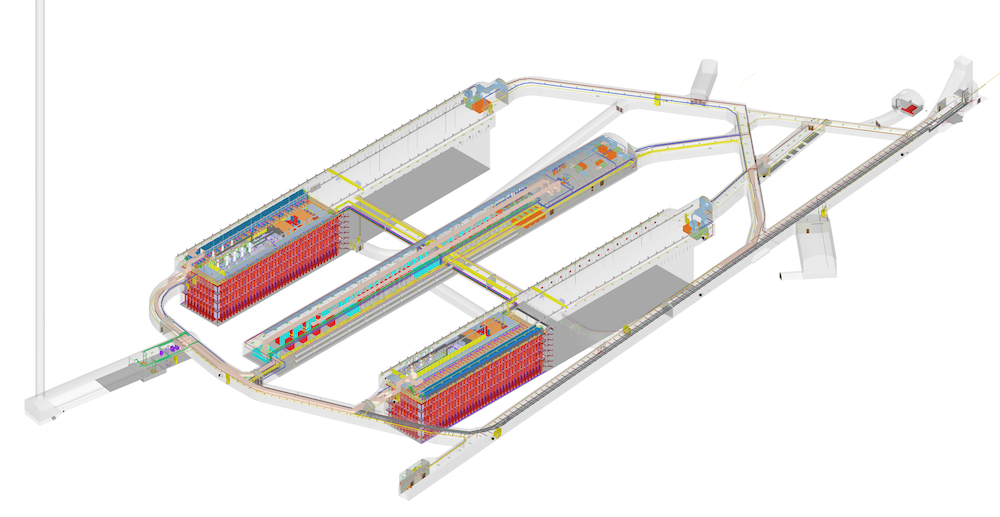
\includegraphics[width=0.7\textwidth]{caverns_full_assembly}
\end{dunefigure}




%%%%%%%%%%%%%%%%%%%%%%%%%%%%%%%%%%%%%%%%%%%%%%%%%%%%%%%%%%%%%%%
\section{The DUNE Detectors}

%The \dword{dune} experiment includes a \dword{nd} at the edge of the \dword{fnal} site, in Batavia, Illinois, and a very large, modular \dword{fd} approximately \SI{1.5}{km} underground at \dword{surf} in Lead, South Dakota, \SI{1300}{km} (\SI{800}{miles}) from \dword{fnal}. The \dword{dune} \dword{fd} is the focus of this \dword{tdr}. 



\subsection{Far Detector}
\label{ch:dune-det-tech-ov-fd}

The \fdfiducialmass \dword{dune} \dword{fd} will consist of four \dword{lartpc} \dwords{detmodule}, each with a \dword{lar} mass in the sensitive region of the cryostat (fiducial mass) of at least \nominalmodsize, installed approximately \SI{1.5}{km} underground. The \dword{lartpc} technology provides
excellent tracking and calorimetry performance, making it an ideal 
choice. Each \dword{lartpc} fits inside a cryostat of internal dimensions
\cryostatwdthinner (w) $\times$ \cryostathtinner (h) $\times$ \cryostatleninner~(l) containing a total \dword{lar} mass of about \larmass{}.
 The design of the four identically sized modules is sufficiently flexible for staging construction and evolving the \dword{lartpc} technology.

\dword{dune} is planning for and currently developing two \dword{lartpc} technologies: \dword{sp} in which all the detector elements inside the cryostat are immersed in liquid; and \dword{dp}, in which some components operate in a layer of gaseous argon above the liquid.

\begin{itemize}
\item In the \dword{sp} technology, ionization charges drift horizontally in the \dword{lar} under the influence of an electric field (\efield) towards %wire planes on 
a vertical anode, where they are read out. 
%The maximum drift length in the first \dword{dune} \dword{spmod} is \spmaxdrift, and the nominal drift field is \spmaxfield, corresponding to a cathode \dword{hv} of \sptargetdriftvoltpos. 
This design requires very low-noise electronics to achieve readout with a good \dword{s/n} ratio because no signal amplification occurs inside the cryostat. 
This technology was pioneered in the \dword{icarus} project, and after several decades of worldwide R\&D, is now mature. It is the technology used for \dword{fnal}'s currently operating \dword{microboone} detector, as well as the \dword{sbnd} detector, which is under construction. Figure~\ref{fig:LArTPC1ch1} shows the operating principle of an \dword{sp} \dword{lartpc}.

\item The \dword{dp} technology was pioneered at a large scale by the \dword{wa105} collaboration at \dword{cern}. It is less mature than the \dword{sp} technology, and whereas it presents some challenges, it offers several advantages.  Here, ionization charges drift vertically upward in \dword{lar} and are transferred into a layer of argon gas above the liquid. Devices called \dwords{lem} amplify the signal charges in the gas phase before they reach a horizontal anode. The gain achieved in the gas reduces the stringent requirements on the electronics noise and the overall design increases the possible drift length, which, in turn, requires a correspondingly higher voltage. %The nominal drift field is \dpnominaldriftfield, as for the \dword{sp} detector, but corresponds to a cathode \dword{hv} of \dptargetdriftvoltpos.
%The maximum drift length in the \dword{dpmod} is \dpmaxdrift{}.  
Figure~\ref{fig:DPprinciplech1} shows the operating principle of a \dword{dp} \dword{lartpc}. 
\end{itemize}
 In both technologies, the drift volumes are surrounded by a \dword{fc} that defines the active detector volume and ensures uniformity of the \efield within that volume.
 
\begin{dunefigure}[The single-phase (SP) LArTPC operating principle]{fig:LArTPC1ch1}
{The general operating principle of the \dword{sp} \dword{lartpc}. Negatively charged ionization electrons from the neutrino interaction drift horizontally opposite to the \efield in the \dword{lar} and are collected on the  %wire planes on 
 anode, which is made up of the U, V and X sense wires.  The right-hand side represents the time projections in two dimensions as the event occurs. Light ($\gamma$) detectors (not shown) will provide the $t_0$ of the interaction.}
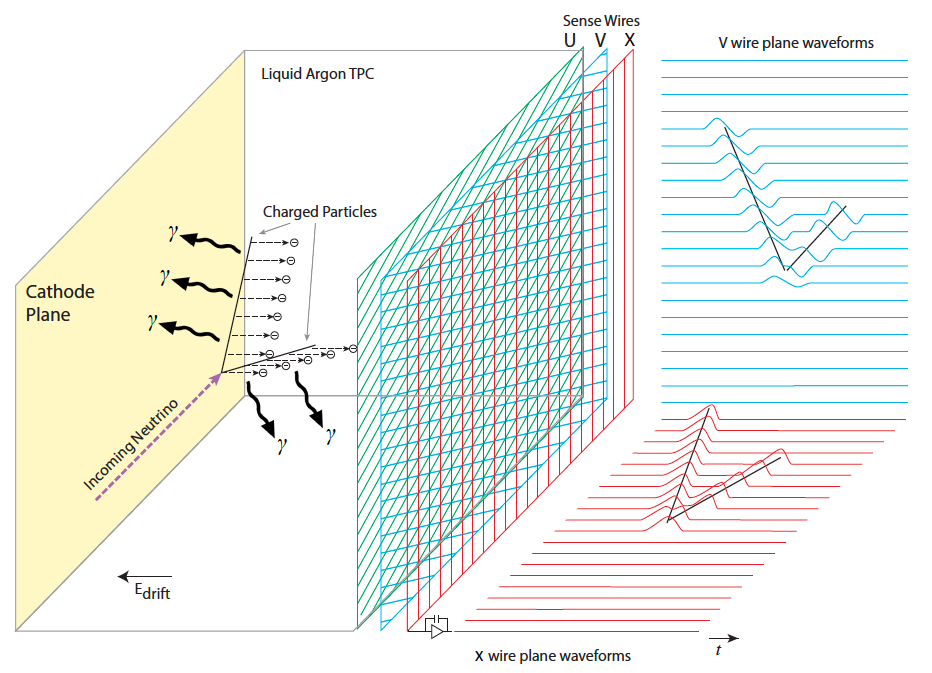
\includegraphics[width=0.75\textwidth]{TheBoPicture.png} 
\end{dunefigure}

\begin{dunefigure}[The dual-phase (DP) LArTPC operating principle]{fig:DPprinciplech1}{The general operating principle of the \dword{dp} \dword{lartpc}. The ionization charges drift vertically upward in \dword{lar} and are transferred into a layer of argon gas above the liquid where they are amplified before collection on the anode. The light detectors (PMTs) sit under the cathode.}
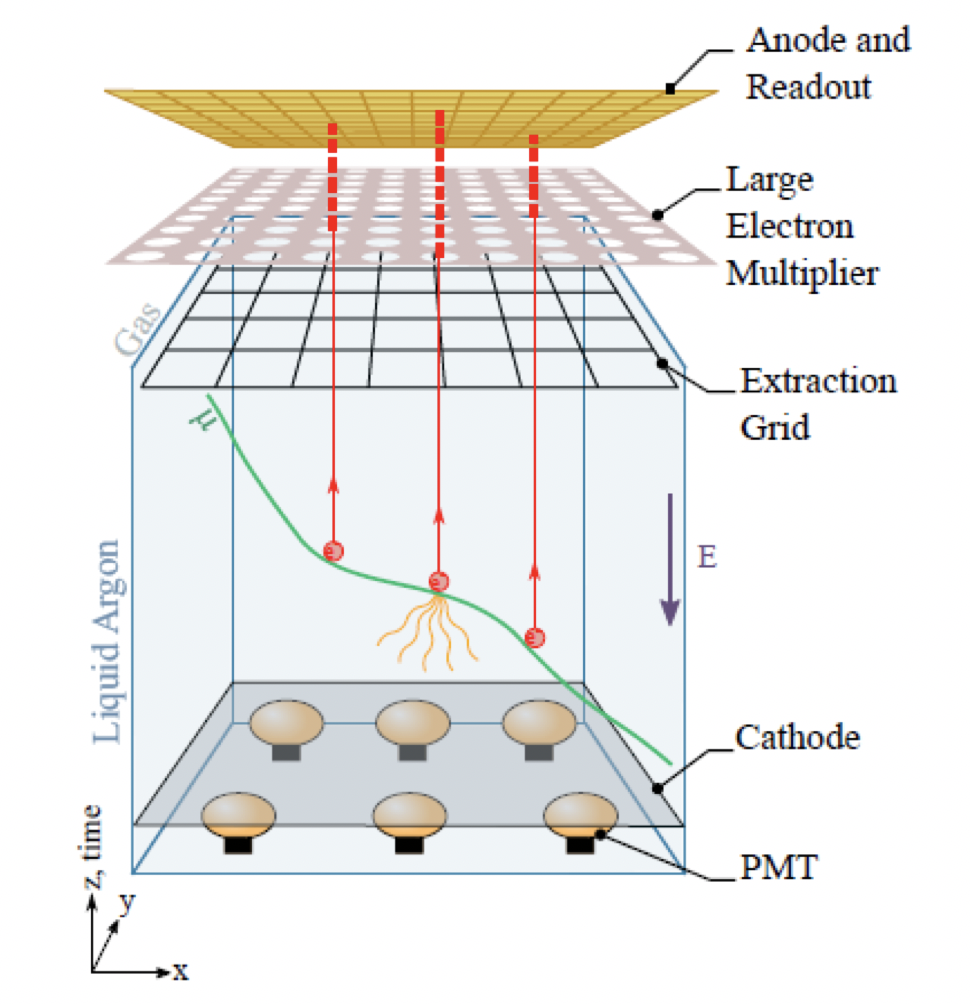
\includegraphics[width=0.5\textwidth]{dualphase-principle}
\end{dunefigure}


Argon is an excellent scintillator at a wavelength of \SI{126.8}{\nano\meter} (UV), a property that both detector designs exploit. This fast scintillation light (photons), once shifted into the visible spectrum, is collected by \dwords{pd} in both designs. The light collection provides an initial start time ($t_{0}$) for every event recorded by the \dword{tpc}, indicating when the ionization electrons begin to drift. Comparing the time at which the ionization signal reaches the anode relative to this start time allows reconstruction of the event topology in the drift coordinate (i.e., horizontal and transverse to the beam for \dword{sp} and vertical for \dword{dp}); the precision of the measured $t_{0}$, therefore, directly corresponds to the precision of the spatial reconstruction in this direction. 

Two key factors affect the performance of the \dword{dune} \dwords{lartpc}, \dword{lar} purity and noise on the readout electronics.  First, the \dword{lar} purity must be %high enough to achieve minimum 
quite high to minimize charge and light attenuation over the longest drift lengths in the \dword{detmodule}.  %Thus, the levels of contaminants (e.g., oxygen, water, and nitrogen) must be maintained at \dword{ppt} levels in the case of oxygen and water and parts per million (ppm) in the case of nitrogen.  
The \dword{sp} and \dword{dp} designs have slightly different purity requirements (expressed in minimum electron lifetimes of \SI{3}{ms} versus \SI{5}{ms}) due to the different maximum drift lengths.
%
Second, the electronic readout of the \dword{lartpc} requires very low noise levels for the signal from the drifting electrons to be clearly discerned over the baseline of the electronics.  This requires using low-noise cryogenic electronics, especially in the case of the \dword{sp} design.

The \dword{dune} collaboration is committed to deploying both technologies. The full \dword{dune} \dword{fd} requires four modules. In this \dword{tdr}, we describe plans for the first three modules: two \dwords{spmod}, one of which will be the first module installed, and one \dword{dpmod}. For planning purposes, we assume that the first \dword{detmodule} will be \dword{sp}, and the second will be \dword{dp}. The actual sequence of \dword{detmodule} installation will depend on results from the prototype detectors, described below, and on available resources. Plans for the fourth \dword{detmodule}, which may use a more advanced design, remain to be determined. 

The plans for the \dword{sp} and \dword{dp} modules are described briefly in the following sections, more fully in Chapters~\ref{ch:exec-sp} and~\ref{ch:exec-dp}, and finally in great detail in Volumes~\volnumbersp{} and~\volnumberdp{} of this \dword{tdr}. 


%%%%%%%%%%%%%%%%%%%%%%%%%%%%%%%%%%%%%%%%
\subsubsection{A Single-Phase Far Detector Module}
\label{sec:fdsp-exec-splar}

The operating principle of an \dword{sp} \dword{lartpc} (Figure~\ref{fig:LArTPC1ch1}) has been demonstrated by  \dword{icarus}~\cite{Icarus-T600}, \dword{microboone}~\cite{microboone}, \dword{argoneut}~\cite{Anderson:2012vc}, \dword{lariat}~\cite{Cavanna:2014iqa}, and \dword{pdsp}~\cite{Abi:2017aow}. Charged particles passing through the \dword{tpc} ionize the argon, and the ionization electrons drift in an \efield{} to the anode planes. Figure~\ref{fig:DUNESchematic1ch1} shows the configuration of a \dword{dune} \dword{spmod}. Each of the four drift volumes of \dword{lar} is subjected to a strong \efield{} of \spmaxfield, corresponding to a cathode \dword{hv} of \sptargetdriftvoltpos. The maximum drift length is \spmaxdrift.  


\begin{dunefigure}[A \nominalmodsize DUNE far detector SP module]{fig:DUNESchematic1ch1}
{A \nominalmodsize \dword{dune} \dword{fd} \dword{spmod}, showing the alternating \sptpclen{} long (into the page), \tpcheight{} high anode (A) and cathode (C) planes, as well as the \dword{fc} that surrounds the drift regions between the anode and cathode planes. On the right-hand cathode plane, the foremost portion of the \dword{fc} is shown in its undeployed (folded) state.}
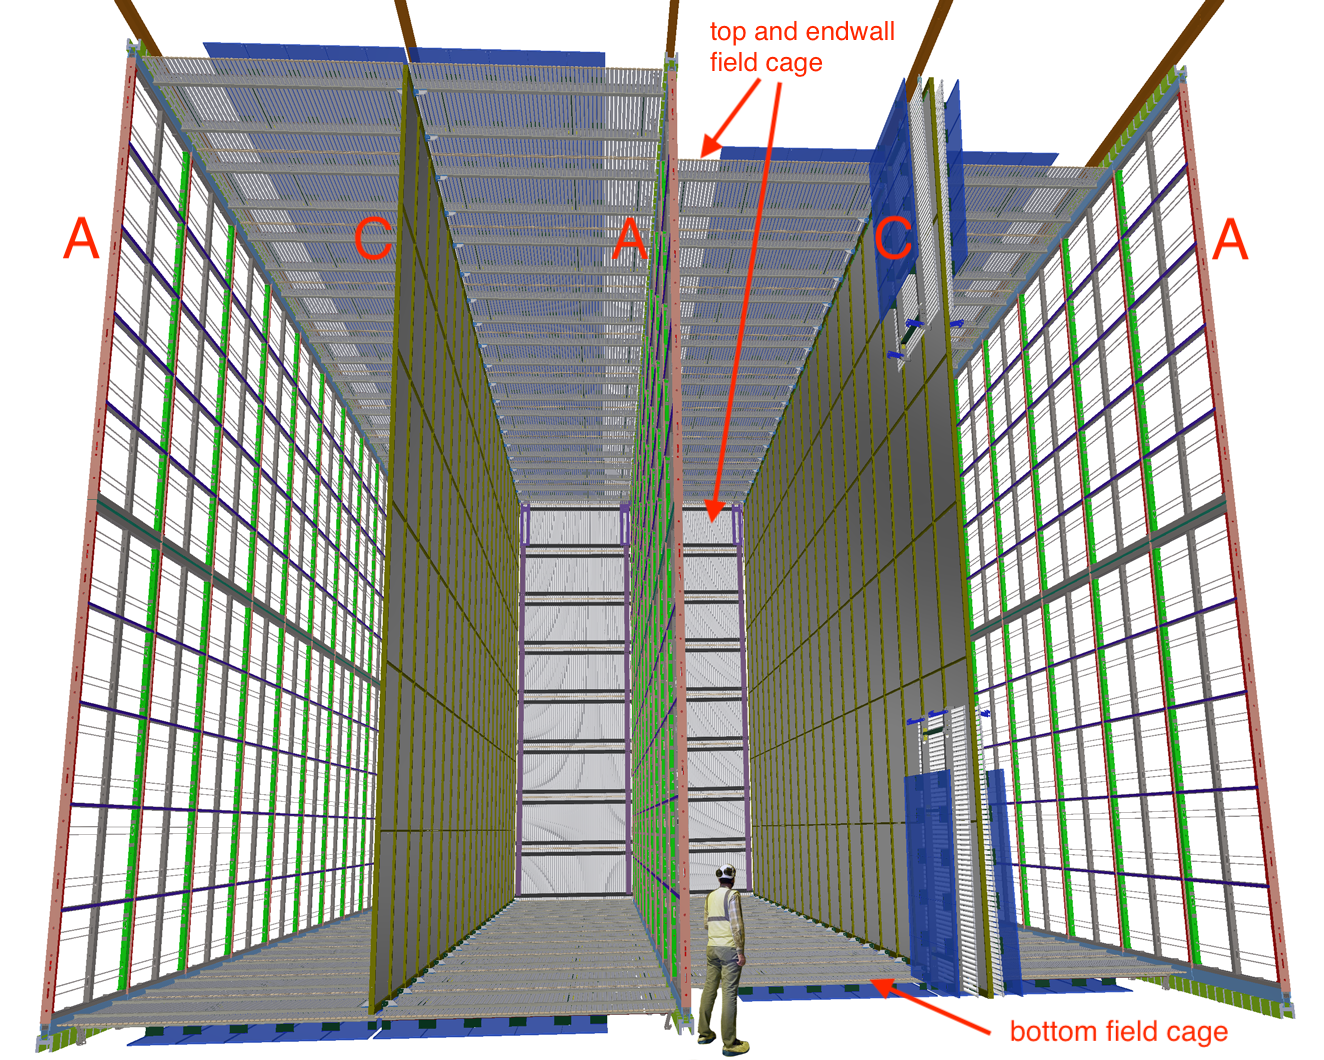
\includegraphics[width=0.65\textwidth]{DUNESchematic.png}
\end{dunefigure}

An \dword{spmod} is instrumented with three module-length (\sptpclen) anode planes constructed from \SI{6}{m} high by \SI{2.3}{m} wide \dwords{apa}, stacked two \dword{apa}s high and 25 wide, for 50 \dword{apa}s per plane, and 150 total. Each \dword{apa} %is two-sided with 
consists of an alumninum frame with three layers of active wires, strung at angles chosen to reduce ambiguities in event reconstruction, to form a grid on each side of the \dword{apa}. The relative voltage between the layers is chosen to ensure transparency to the drifting electrons of the first two layers ($U$ and $V$). These layers produce bipolar induction signals as the electrons pass through them. The final layer ($X$) collects the drifting electrons, resulting in a unipolar signal. The pattern of ionization collected on the grid of anode wires provides the reconstruction in the remaining two coordinates perpendicular to the drift direction (Figure~\ref{fig:LArTPC1ch1}).

Novel \dword{sipm} based \dfirsts{pd} called ARAPUCAs are placed in the inactive space between the innermost wire planes of the \dword{apa}s, installed through slots in the \dword{apa} frame. 
Each \dword{apa} holds ten \dword{pd} modules, for a total of \num{1500} per \dword{spmod}.  Of these, \num{500} are mounted in the \dword{apa}s of the central anode plane and collect light from both directions, 
and \num{500} each are mounted in the outer \dword{apa} frames and collect light from only the inner-facing direction. 

%% anne here 12/10
\FloatBarrier
%%%%%%%%%%%%%%%%%%%%%%%%%%%%%%%%%%%%%%%%
\subsubsection{A Dual-Phase Far Detector Module}
\label{sec:fddp-exec-splar}

The \dword{dp} operating principle, illustrated in Figure~\ref{fig:DPprinciplech1}, is very similar to that of the \dword{sp}. % design. 
 Charged particles that traverse the active volume of the \dword{lartpc} ionize the medium while also producing scintillation light.  The ionization electrons drift, in this case vertically, along an \efield toward a segmented anode where they deposit their charge. Any scintillation light that is produced is measured in  \dwords{pd} that view the interior of the volume from below. 
 
 

%The key differentiating concept of the \dword{dp} design is the amplification of the ionization signal in an avalanche process that takes place in a layer of argon gas above the \dword{lar}.  
In this design, shown in Figure~\ref{fig:DPdet1ch1}, ionization electrons drift upward toward an extraction grid just below the liquid-vapor interface. 
After reaching the grid, an \efield stronger than the \dpnominaldriftfield{} drift field extracts the electrons from the liquid up into the gas phase. Once in the gas, the electrons encounter micro-pattern gas detectors, called \dwords{lem}, with high-field regions
in which they are amplified. 
%. The \dwords{lem} amplify the electrons in avalanches that occur in these high-field regions. 
The amplified charge is then collected and recorded on a \twod anode
consisting of two sets of %\SI{3.125}{mm}-pitch 
gold-plated copper strips that provide the $x$ and $y$ coordinates (and thus two views) of an event. 
An array of \dwords{pmt} coated with a wavelength-shifting material sits below the cathode to record the time ($t_{0}$) and pulse characteristics of the incident light.


\begin{dunefigure}[A \nominalmodsize DUNE far detector DP module]{fig:DPdet1ch1}
  {Schematic of a \nominalmodsize \dword{dune} \dword{fd} \dword{dp} \dword{detmodule} with cathode, \dwords{pmt}, \dword{fc}, and anode plane with \dwords{sftchimney}. The drift direction is vertical in the case of a DP module.}
  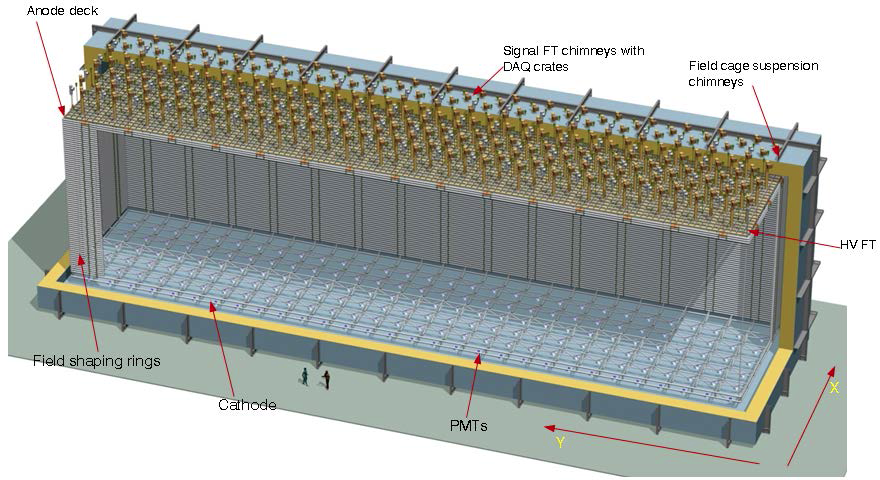
\includegraphics[width=0.9\textwidth]{DUNE-CDR-detectors-volume-optim.png}
\end{dunefigure}

The extraction grid, \dword{lem}, and anode are assembled into three-layered \textit{sandwiches} with precisely defined inter-stage distances and inter-alignment,  which are then connected horizontally into \num{9}~m$^2$ modular detection units called \dwords{crp}.

The precision tracking and calorimetry offered by both the \dword{sp} and \dword{dp} technologies provide excellent capabilities for identifying interactions of interest while mitigating sources of background.  Whereas the \dword{sp} design has multiple drift volumes, the \dword{dpmod} design allows a single, fully homogeneous \dword{lar} volume with a much longer drift length.

\FloatBarrier

%%%%%%%%%%%%%%%%%%%%%%%
\subsubsection{ProtoDUNEs: Far Detector Prototypes}

The \dword{dune} collaboration has constructed and operated 
two large prototype detectors, \dword{pdsp}, and \dword{pddp}, at \dword{cern}.  %one using \single readout (\dword{pdsp}) and the other \dual readout (\dword{pddp}).
 Each is approximately one-twentieth the size of the planned \dword{fd} modules but uses components identical in size to those of the full-scale module. \dword{pdsp} has the same \spmaxdrift maximum drift length as the full \dword{spmod}. \dword{pddp} has a \SI{6}{m} maximum drift length, half that planned for the \dword{dpmod}.  Figure~\ref{fig:protodunes_northarea} shows the two cryostats, \dword{pdsp} in the foreground and \dword{pddp} at an angle in the rear. Figure~\ref{fig:protodunes_interior} shows one of the two drift volumes of \dword{pdsp} on the left and the single drift volume of \dword{pddp} on the right.

\begin{dunefigure}[ProtoDUNE cryostats at the CERN Neutrino Platform]
{fig:protodunes_northarea}
{\dword{pdsp}{} and \dword{pddp}{} cryostats in the \dword{cern}{} Neutrino Platform in \dword{cern}'s North Area.}
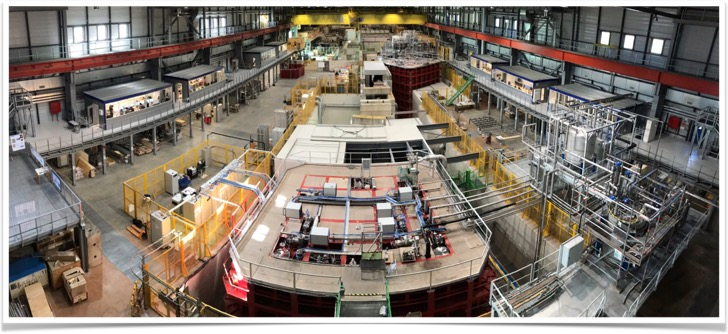
\includegraphics[width=0.9\linewidth]{neutrinoplatform.jpg}
\end{dunefigure}

\begin{dunefigure}[Interior views of the ProtoDUNEs]
{fig:protodunes_interior}
{Left: View of one of the two drift volumes in \dword{pdsp}; the \dword{apa} is on the left, the \dword{cpa} is on the right, and two of the four the \dword{fc} surfaces bounding the drift volume are at the center and bottom of the image.  Right:  the single \dword{pddp} drift volume (still incomplete when the image was taken), looking up; the \dwords{crp} (orange) are at the top. Three sides of the surrounding \dword{fc} are shown, but the cathode is not visible.}
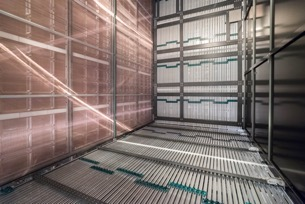
\includegraphics[width=0.46\linewidth]{graphics/ProtoDUNE-sp-interior.jpg}\hspace{0.05\linewidth}
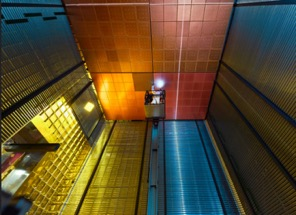
\includegraphics[width=0.44\linewidth]{graphics/protodune-dp-interior.jpg}
\end{dunefigure}

This massive prototyping program was undertaken with both engineering and scientific goals in mind, namely: 
 
\begin{enumerate}
\item production of components: stress-test the production and \dword{qa} processes of detector components and mitigate the associated risks for the \dword{fd};
\item validation of installation procedures: test the interfaces between the detector elements
and mitigate the associated risks for the \dword{fd};
\item operation of the detector with cosmic rays: validate the detector designs and performance; and 
\item collection of test beam data: measure the physics response of the detector.
\end{enumerate}

%The \dword{protodune} program has in fact succeeded in allowing us to accomplish these goals and validate key aspects of the \dword{tpc} designs. %, test engineering procedures, and collect valuable calibration data. %We were able to run \dword{pdsp}) in a hadron test beam. 

Construction of the \dword{pdsp} detector was finished in July 2018 and filled with \dword{lar} the following month. It collected hadron beam and cosmic ray data during the fall of 2018 and continues to collect cosmic ray data.  Construction of the \dword{pddp} detector was complete in June of 2019, and the detector started operations in September 2019.

The data taken with \dword{pdsp} demonstrate the detector's excellent performance and have already provided valuable information on the design, calibration, and simulation of the \dword{dune} \dword{fd}. In all, $99.7\%$ of the 15360 \dword{tpc} electronics channels are responsive in the \dword{lar}. The \dword{enc} amounts to $\approx 550$ $e^{-}$ on the collection wires and $\approx 650$ $e^{-}$ on the induction wires, roughly half of the allowed maximum. An average \dword{s/n} of 38 for the collection plane is measured using cosmic-ray muons, while for the two induction planes, the \dword{s/n} is 14 (U) and 17 (V), easily exceeding the requirement of 4 %a ratio $9/1$ 
for the \dword{dune} \dword{fd}. 

\fixme{I took out a pgraph about the space charge effect and dE/dx distributions- it's too much for our targeted audience IMHO. Could be in SP chapter maybe. Need to remove fig 11 left, too. Anne}
%Because \dword{pdsp} is located on the surface,  an excess of ions accumulates in the drift volume, % that distorts  distorting the \efield and the reconstructed particle trajectories; this is known as the \textit{space charge effect}. 
%A calibration procedure removes the detector non-uniformity, which is dominated by this effect.  We then convert the charge deposited along the track to the energy loss ($dE/dx$) using stopping cosmic ray muons. The calibration constants that have been derived with this method are applied to the energy deposits measured for the beam particles, including muons, pions, protons, and positrons.The resulting $dE/dx$ distributions agree well with expectations.  Figure~\ref{fig:pdtpcpd} (left) shows the calibrated $dE/dx$ values as a function of the track residual range for protons in the 1 GeV/$c$ beam, in good agreement with expectations. 



The \dword{pdsp} beam run provides a unique set of high-quality data for detector performance characterization, physics studies, and calibration, and will 
allow us to perform hadron-argon cross section measurements, which are relevant for future \dword{dune} neutrino oscillation analyses.
Data collected during the beam run will also be used to characterize the \dword{pds} response to light signals. Other useful data sets include
beam data with triggers determined by the beam instrumentation; cosmic ray data  from random triggers or from those in coincidence with the \dword{crt} modules; and calibration data, with triggers enabling programmed light pulses. 
The %single avalanche    --- it's not explained anywhere
response and gain for each of the 256 readout channels of the \dword{pds} have been determined from calibration data, and 
the initial analysis results indicate very good performance and stability for this system. 

Figure~\ref{fig:pdtpcpd} (right) shows the response of an %ARAPUCA photon-detector 
ARAPUCA \dword{pd} module (not corrected for geometry and detection efficiency) as a function of incident electron kinetic energy measured by a \dword{tpc}. \fixme{but this was not protodune sp?}
%The observed number of photons has 
 This preliminary analysis demonstrates the achieved energy linearity for beam electrons contained in the detector.  
In addition to verifying the \dword{pds} response and calibration, \dword{pdsp} showed excellent correlation between \dword{tpc} timing and the \dword{pds} timing. The latter will enable the further optimized physics reach of \dword{dune}. 

\fixme{I have removed the left figure assuming we remove the paragraph above. Anne}

  \begin{comment}  %%%% replaced below
  [Calibrated $dE/dx$ vs residual range in ProtoDUNE-SP]
  {fig:pdtpcpd}
  {Left: Calibrated $dE/dx$ (energy loss over distance) versus residual range measured by a \dword{tpc} for 1 GeV/c   
  stopping protons. Right: Response in \dword{pdsp} of an ARAPUCA \dword{pd} module in \dword{apa}{}3 as a function of 
  incident electron kinetic energy.} 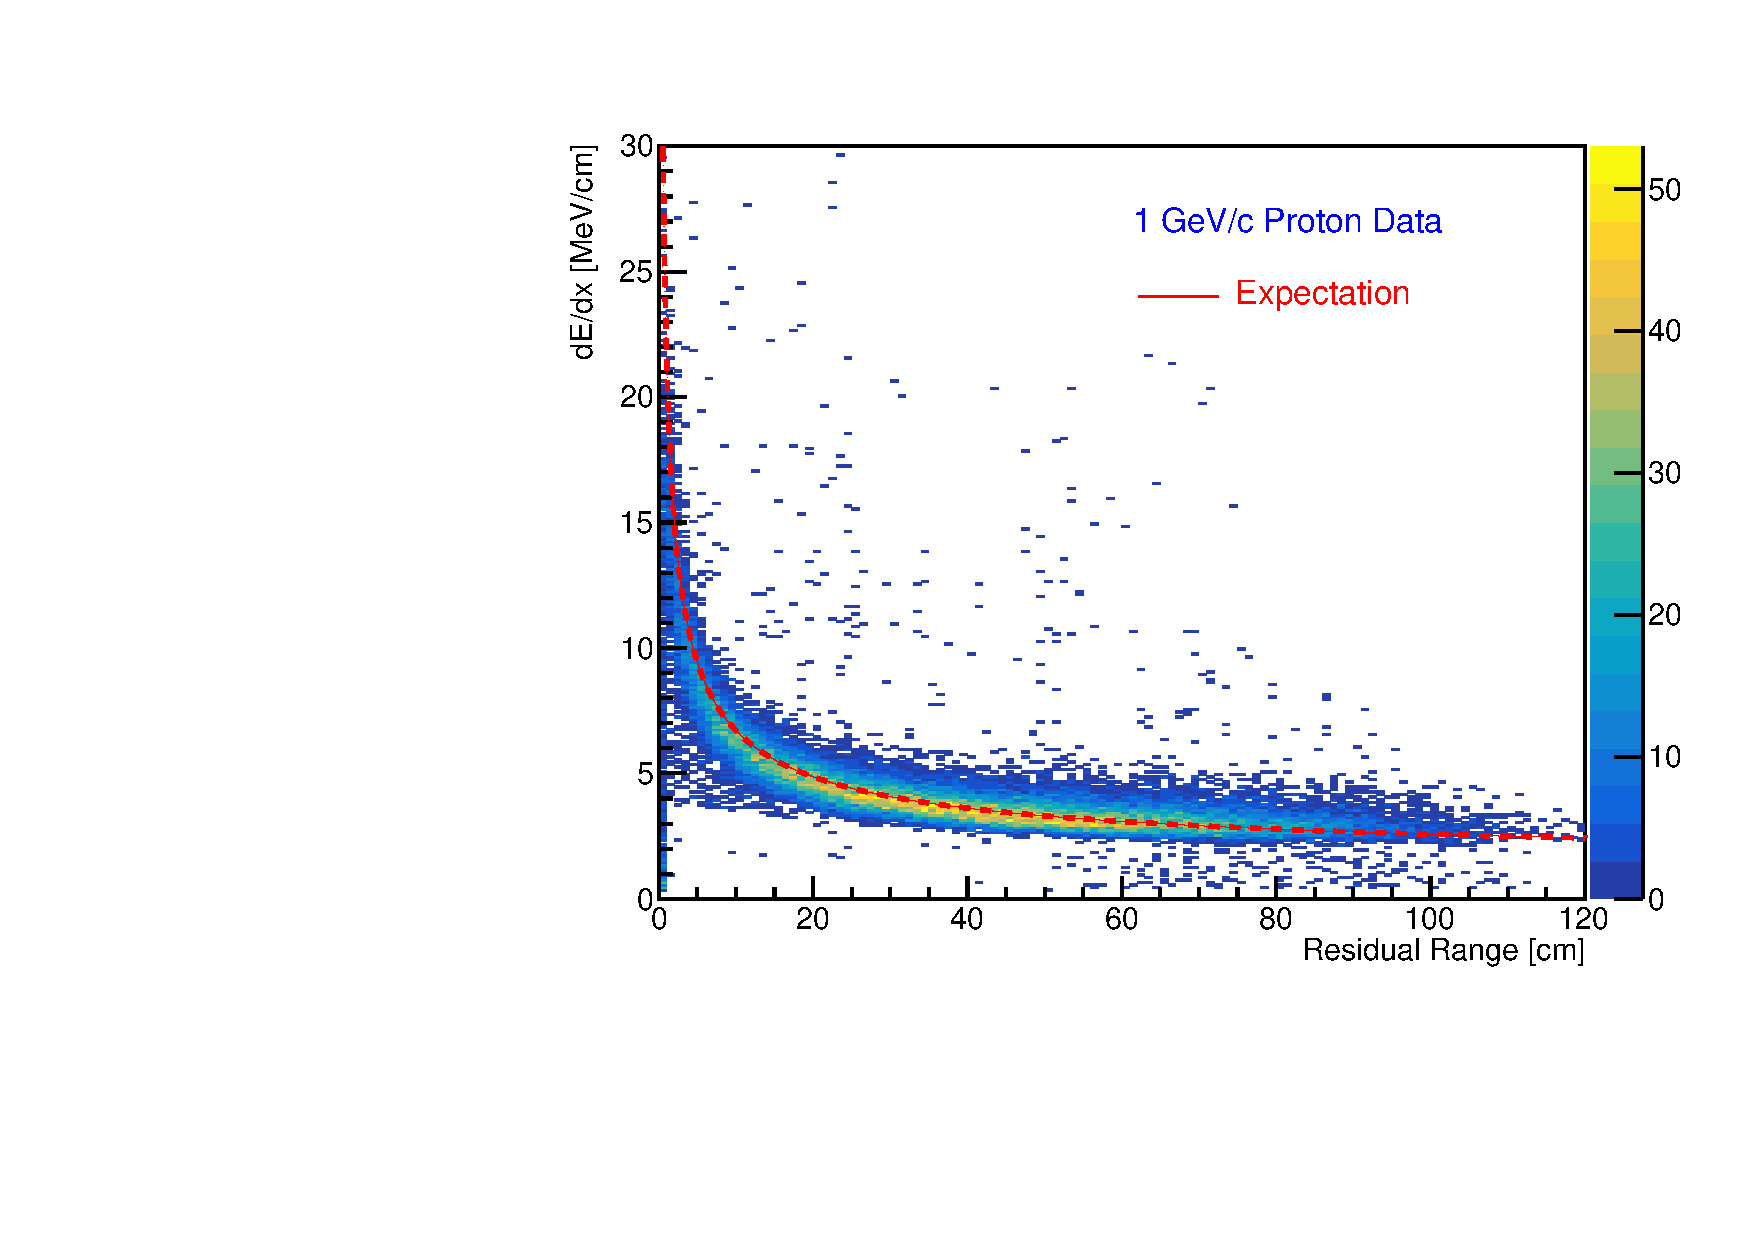
\includegraphics[width=0.47\linewidth]{graphics/dedx_rr_data_v5.pdf}
  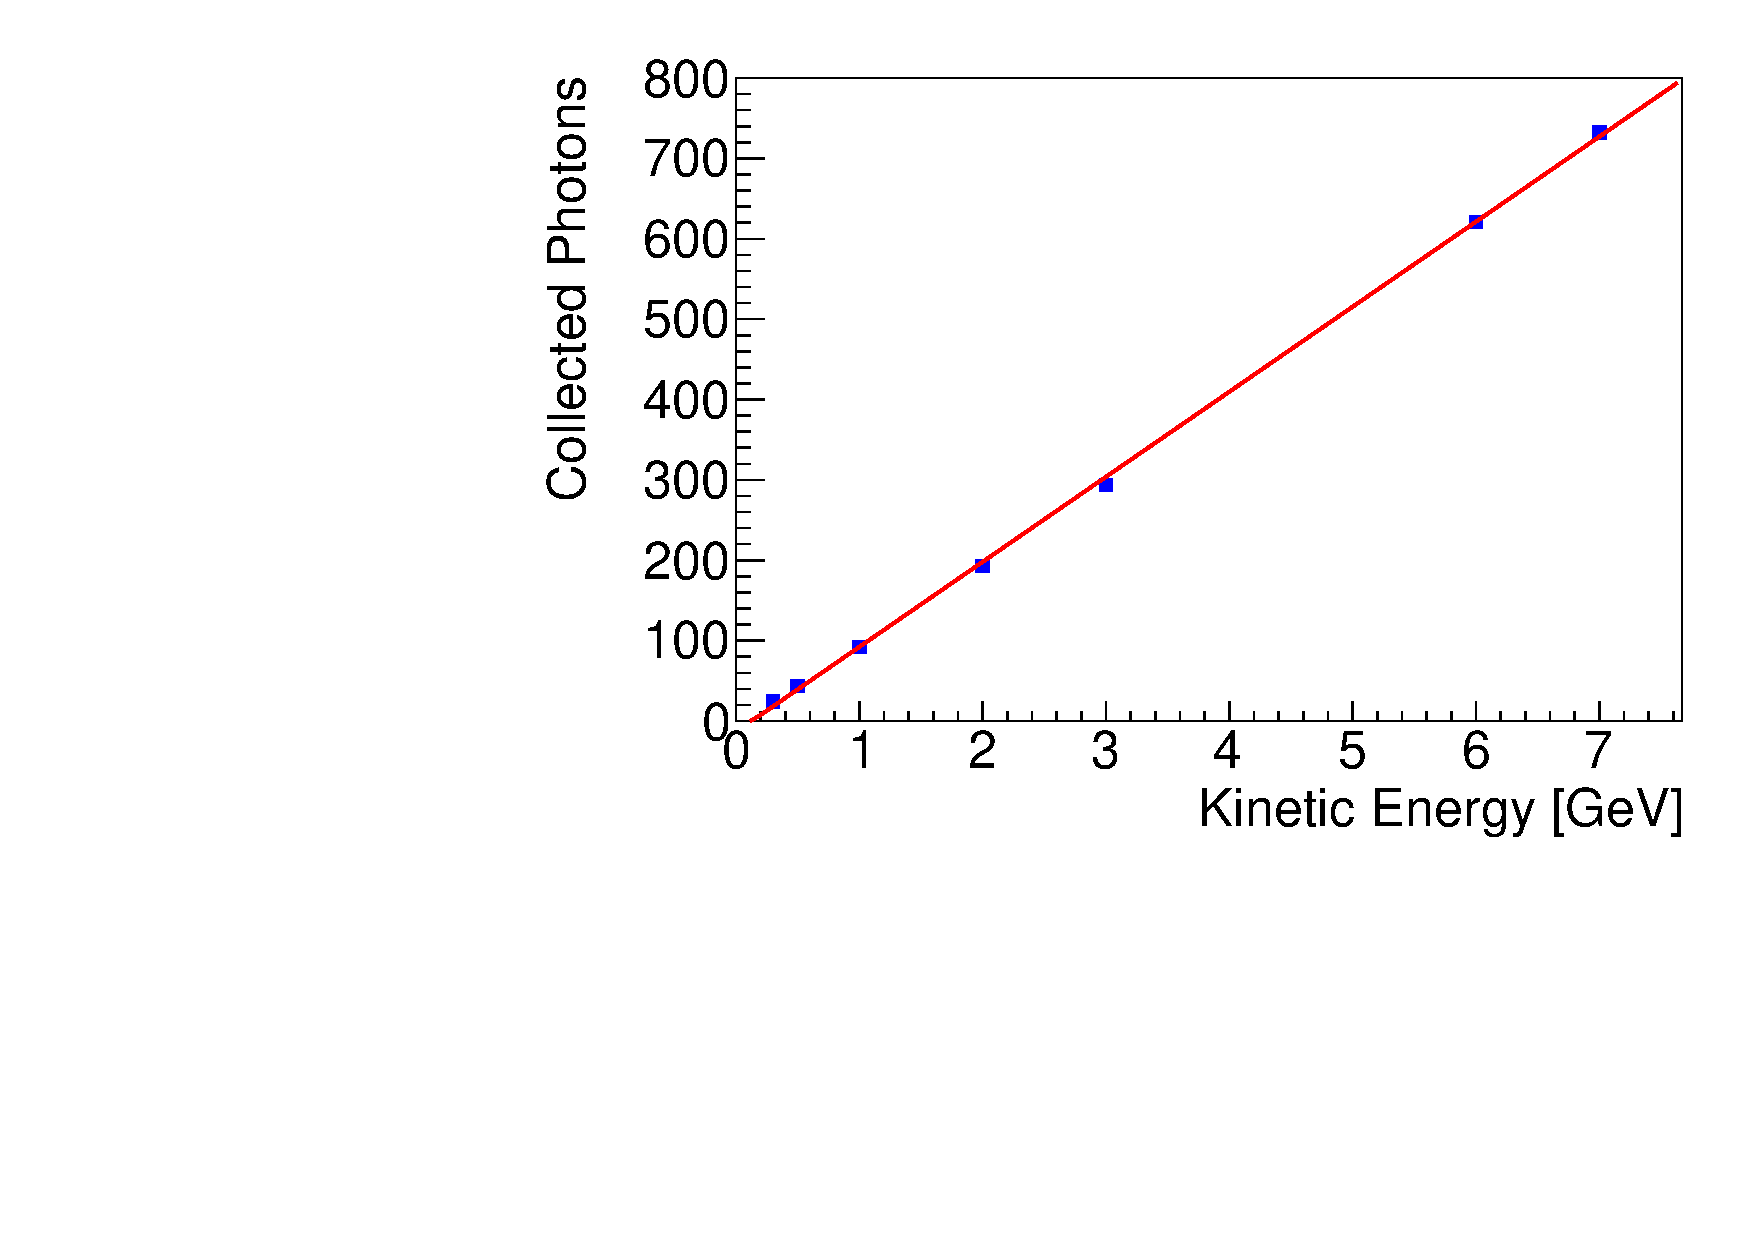
\includegraphics[width=0.5\linewidth]{pdsarapucabeamresponse.pdf}
  \end{comment}
  
\begin{dunefigure}[Response in \dshort{pdsp} of an ARAPUCA \dshort{pd} module]
{fig:pdtpcpd}
{Response in \dword{pdsp} of an ARAPUCA \dword{pd} module in \dword{apa}{}3 as a function of incident electron kinetic energy.} 

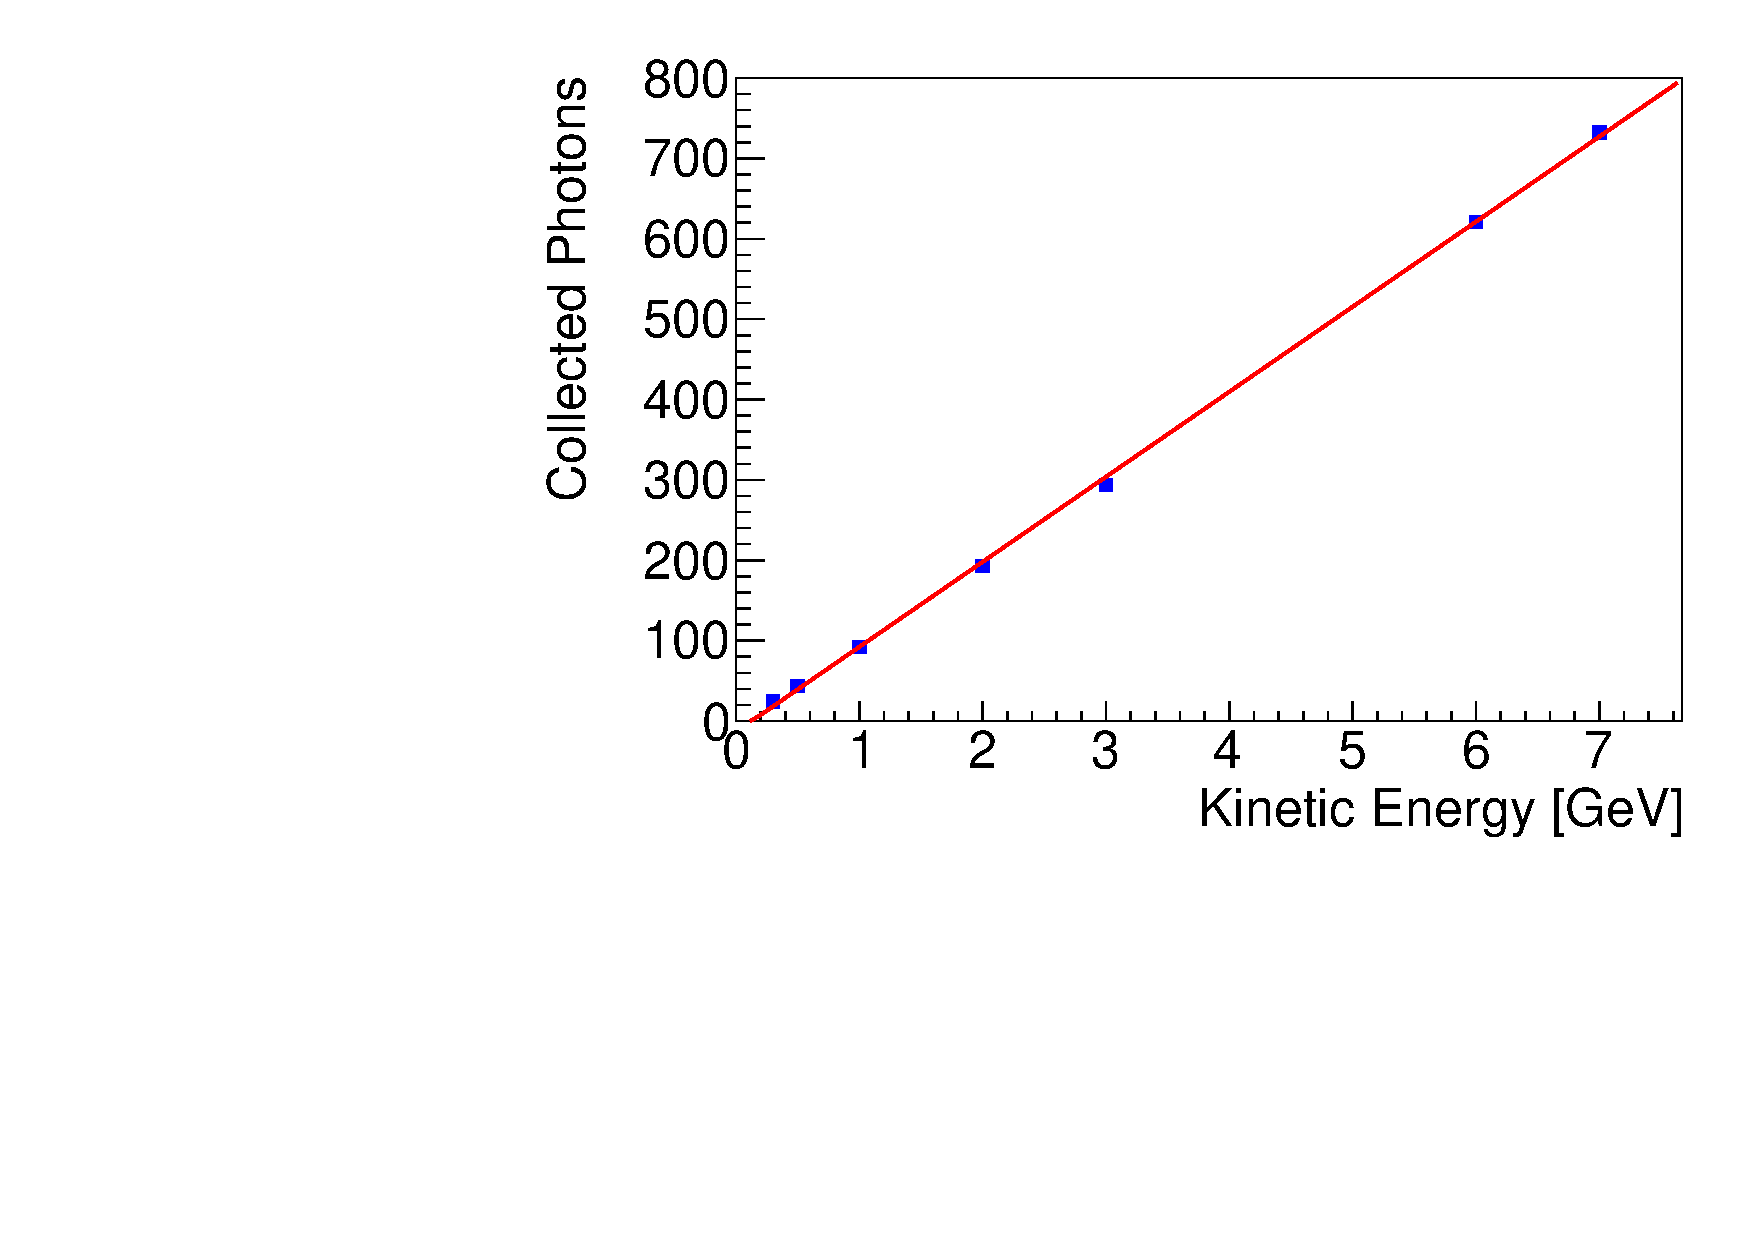
\includegraphics[width=0.65\linewidth]{pdsarapucabeamresponse.pdf}
\end{dunefigure}

\fixme{Can we say a bit more about PDUNE-DP and what we've learned?}

%%%%%%%%%%%%%%%%%%%%%%%%%%%%%%%%%%%%%%%%%%%%%%
\subsection{Near Detector}
\label{sec:nd-verview}

Although not the subject of this \dword{tdr}, an understanding of \dword{dune}'s capabilities would be impossible without 
some description of the crucial contribution of the \dword{nd} to the experiment.
%The \dword{dune} \dword{nd} is crucial for the success of the \dword{dune} physics program. It 
The \dword{nd} will serve as the experiment's control,
 constraining systematic errors and measuring the initial unoscillated \numu and \nue energy spectra (and that of the corresponding antineutrinos). 
%A key role it plays regarding neutrino oscillation physics is to precisely measure the neutrino beam flux and flavor composition near the beam source, before any oscillation takes place. 
Comparing the measured neutrino energy spectra near the beam source, before any oscillation takes place, and again at the far site allows us to disentangle the different energy-dependent effects that modulate the beam spectrum and to reduce the systematic uncertainties to the level required for discovering \dword{cpv}. Its other key role in this arena is to measure neutrino-argon interactions with high precision using both gaseous and liquid argon, which will further reduce the systematic uncertainties associated with modeling these interactions. 

The \dword{nd} will have a physics program of its own, as well, independent of the \dword{fd}.  This program will include measuring neutrino interactions to explore the two pillars of the standard model: electroweak physics and quantum chromodynamics. It will also explore physics beyond the standard model, searching for non-standard interactions, sterile neutrinos,  dark photons, and  other exotic particles.

The \dword{nd} will be located \SI{574}{m} downstream from the neutrino beam source and will include three primary detector components, shown in Figure~\ref{fig:neardetectors}. Two of them can move off axis relative to the beam, providing access to different neutrino energy spectra. The movement off axis, called \dword{duneprism}, provides a crucial extra degree of freedom for the \dword{nd} measurements and is an integral part of the \dword{dune} \dword{nd} concept. 


\begin{dunefigure}[DUNE near detector (ND)]
{fig:neardetectors}
{\dword{dune}{} Near Detector. The beam enters from the right and encounters
the \dword{lartpc}, the \dshort{mpd}, and the on-axis beam monitor.}
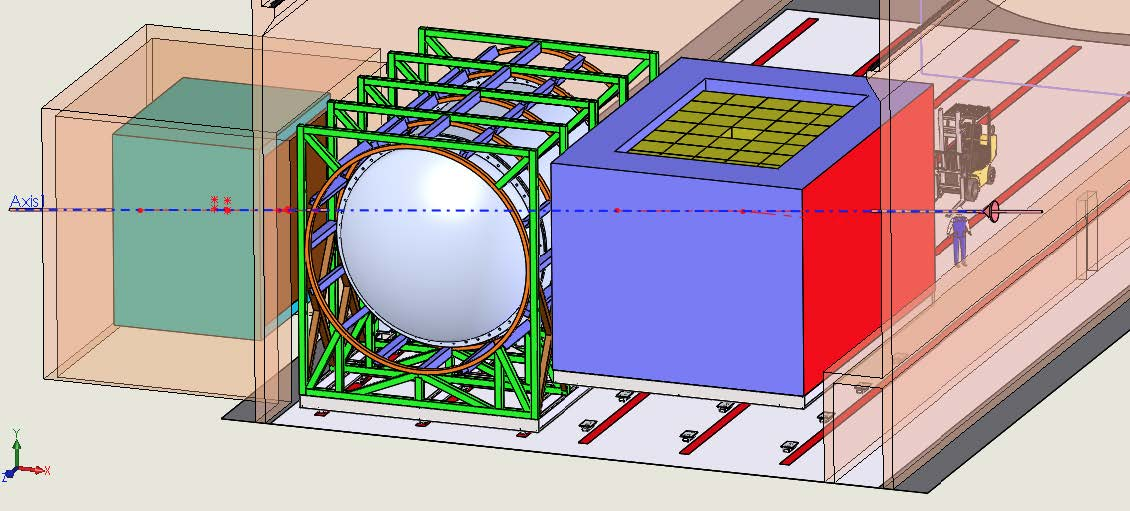
\includegraphics[width=0.9\textwidth]{ND_Detectors.jpg}
\end{dunefigure}

The three detector components are
\begin{itemize}
\item a \dword{lartpc} called \dword{arcube}; 
\item a \dword{hpgtpc} surrounded by an \dword{ecal} in a \SI{0.5}{T} magnetic field, together called the \dword{mpd}; and 
\item an on-axis beam monitor. % containing a \dword{3dst} surrounded by the KLOE magnet.
\end{itemize}
They serve important individual and overlapping functions in the mission of the \dword{nd}. 




The \dword{arcube} detector contains the same target nucleus and shares some aspects of form and functionality with the \dword{fd}. 
%The differences are necessitated by the expected high intensity of the neutrino beam at the \dword{nd}.  
This similarity in target nucleus and, to some extent, technology, reduces sensitivity to nuclear effects and detector-driven systematic uncertainties in extracting the oscillation signal at the  \dword{fd}. %Using the same target nucleus is particularly important because extrapolation of cross sections between nuclear targets with different atomic number is highly model-dependent. 
\dword{arcube} is large enough to provide high statistics ($\num{1e8}$ ${\numu \text{ charged current events/year}}$ on-axis), and its volume is sufficiently large to provide good hadron containment.  The tracking and energy resolution, combined with the \dword{lar} mass, will allow measuring the flux in the beam using several techniques. %, including the well understood but rare process of $\nu$+e$^{-}$ scattering.

\begin{dunefigure}[DUNE ND hall with component detectors]
{fig:NDHallconfigs}
{\dword{dune} \dword{nd} hall shown with component detectors all in the on-axis configuration (left) and with the \dword{lartpc} and \dword{mpd} in an off-axis configuration (right). The %\dword{3dst} spectrometer 
beam monitor (\dshort{3dsts}) is shown in position on the beam axis in both figures. The beam is shown entering the hall at the bottom traveling from right to left.}
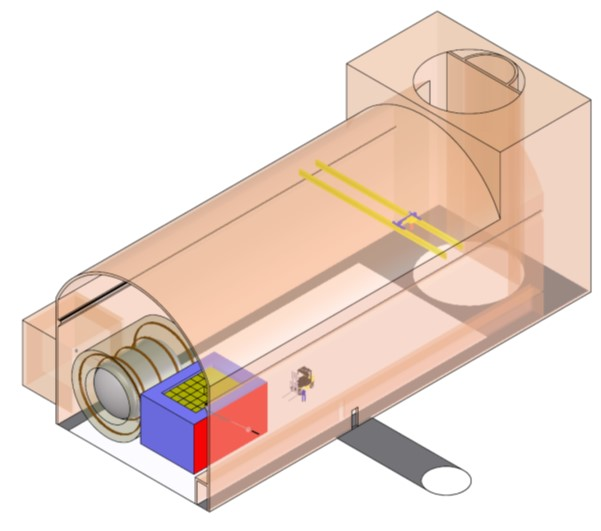
\includegraphics[width=0.49\textwidth]{graphics/NDHall_onaxis.jpg}
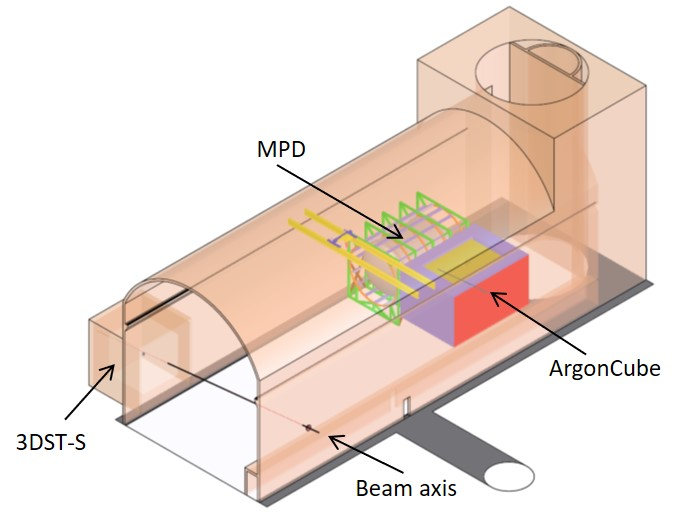
\includegraphics[width=0.49\textwidth]{graphics/NDHall_offaxis.jpg}
\end{dunefigure}

A \dword{lartpc} begins to lose acceptance for muons with a measured momentum higher than $\sim0.7$~GeV/c because the muons will not be contained in the \dword{lartpc} volume.  Because muon momentum is critical to determining the incoming neutrino's energy, a magnetic spectrometer is needed downstream of the \dword{lartpc} to measure the momentum and charge of the muons.  %Measuring  the charge of the muons is particularly important in antineutrino running given that the beam will be an admixture of neutrinos and antineutrinos. 
In the \dword{dune} \dword{nd} concept, the \dword{mpd} will make these measurements. The \dword{hpgtpc} provides a lower density medium with excellent tracking resolution for muons from the \dword{lartpc}.  

%Neutrinos interacting with the argon in the gas \dword{tpc} constitute a sample of $\nu$-argon events that can be studied with a very low charged-particle tracking threshold and excellent resolution superior to \dword{lar}. The high pressure yields a sample of $\num{2e6}$ $\numu$ charged current events/year on-axis for these studies. These events will be valuable for studying charged particle activity near the interaction vertex because this detector can access lower momenta protons than the \dword{lar} detector and can better identify charged pions.  The gas TPC can also provide a separate measurement of $\nu_e$ and $\overline{\nu_e}$ in the beam. In addition, the lack of secondary interactions in these neutrino samples will help in identifying the particles produced in the primary interaction and in modeling secondary interactions in denser detectors, which are known to be important \cite{Friedland:2018vry}.

The \dword{lartpc} and \dword{mpd} can be moved sideways up to \SI{33}{m} to take data in positions off the beam axis (\dword{duneprism}). As the detectors move off-axis, the incident neutrino flux spectrum changes, with the mean energy dropping and the spectrum becoming more monochromatic.  %Although the neutrino interaction rate drops off-axis, the intensity of the beam and the size of the \dword{lartpc}  combine to yield ample statistics even in the off-axis positions.
The \dword{dune} concept is based on reconstructing the energy-dependent neutrino spectrum and comparing measurements at the far and near sites. The ability to take measurements at the near site in off-axis locations will allow us to 
disentangle otherwise degenerate effects due to systematic biases of the energy reconstruction.

The final component of the \dword{dune} \dword{nd} suite is the on-axis beam monitor.
%, which contains the \dword{3dst} tracker within the KLOE magnet.  The concept for this tracker is a  plastic scintillator detector made of \SI{1}{cm} cubes read out along each of three orthogonal dimensions.  
This device would serve as a dedicated  neutrino spectrum monitor that stays on-axis  when the \dword{lartpc} and \dword{mpd} have moved to an off-axis position. 
It can also provide an excellent on-axis neutrino flux determination that can be used as an important point of comparison and a systematic crosscheck for the flux as determined by the \dword{lartpc}.

%The DUNE collaboration is now in the process of finalizing studies for the ND CDR.  Following completion of the CDR, DUNE plans to form ND consortia charged with delivering the final design of ND elements and developing the responsibility matrix for delivery of this design.  The ND consortia will take a leading role in developing the ND TDR which is planned for completion in 2020.

Chapter~\ref{ch:exsum-nd} of this \dword{tdr} volume presents a more complete introduction to the \dword{nd} and further details of the system can be found in the appendices. The DUNE collaboration is now in the process of finalizing studies for the \dword{nd} Conceptual Design Report.

%%%%%%%%%%%%%%%%%%%%%%%%%%%%%%%%
\section{DUNE Project Organization and Responsibilities} %{International DUNE Project Organization and Responsibilities}
\label{es:ch1:intl-org-resp}

\dword{dune} is the first large-scale science project in the U.S. %of this scale 
to be built %with this level of international participation and 
as a fully international collaboration with majority international participation. As such, \dword{dune} requires a new organizational and governance model that takes into account the international nature of the project and its relationship
to \dword{lbnf}.
The model used by \dword{cern} to manage constructing and operating the \dword{lhc} and its experiments served as a starting point for the %joint 
management structure of  \dword{dune} and \dword{lbnf}, 
and our model continues to evolve as the \dword{dune} project moves forward in concert with \dword{lbnf} to build this experiment and the supporting facilities.  The \dword{dune} project is %a fully international project
organized by the \dword{dune} collaboration (Section~\ref{sec:exec:collab:org}) with appropriate oversight from all international stakeholders. In contrast, 
\dword{lbnf} (Section~\ref{sec:exec:lbnf}) %, which is responsible for the facilities that comprise the neutrino beam, the near site at \dword{fnal}, and the far site at \surf{}, 
is organized as a \dword{doe}-\dword{fnal} project incorporating international partners. 

%  The \dword{dune} collaboration is responsible for:
%  \begin{itemize}
%  \item the definition of the scientific goals and corresponding scientific and technical requirements of the detector systems and neutrino beamline;
%  \item the design, construction, commissioning, and operation of the detectors; and
%  \item the scientific research program conducted with the \dword{dune} detectors. 
%  \end{itemize}

A set  of  organizational structures  has been established  to
coordinate  the  participating  funding agencies,
overseeing the \dword{lbnf} and \dword{dune} projects,
and coordinating and communicating between the 
two. These structures and the relationships among them are shown 
in Figure~\ref{fig:org}. They include %comprise 
the following committees:
\begin{itemize}
\item International Neutrino Council 

The \dword{inc} is part of the international project governance structure for the  \dword{lbnf} and the  \dword{pip2} projects. The \dword{inc} comprises representatives from the international funding agencies and  \dword{cern} that make major contributions to the infrastructure. 
The \dword{inc} acts as the highest-level international advisory body to the U.S.  \dword{doe} and the  \dword{fnal} directorate on anything related to the program, including coordination among the international partners. The associate director for HEP in the \dword{doe} Office of Science chairs the \dword{inc}, and the \dword{inc}{} includes the  \dword{fnal} director as a member. The council meets once a year and provides pertinent advice on the \dword{lbnf} and \dword{pip2}  projects.

\item Resources Review Board (RRB)

A \dword{rrb} is part of \dword{dune}'s international project governance structure, % for the   experiment, 
established to coordinate among funding partners and oversee the \dword{dune} project. It includes representatives from all funding agencies that sponsor the project and  from \dword{fnal} management. The  \dword{rrb} provides focused monitoring of the \dword{dune} collaboration and also receives updates on the progress of \dword{lbnf},  \dword{pip2}, and the \dword{sbn} programs. The  \dword{rrb} receives periodic reports from both \dword{lbnc} and \dword{ncg}, described here. %, which are review committees for \dword{dune} charged by and reporting to the \dword{fnal} directorate. 
A representative from the \dword{fnal} directorate chairs the \dword{rrb} and calls regular meetings to monitor progress on the \dword{dune} project.



\item Long-Baseline Neutrino Committee (LBNC)

The \dword{fnal} director has charged the \dword{lbnc} to review the scientific, technical, and managerial progress, as well as plans and decisions associated with the \dword{dune} project. %The committee chair reports to the \dword{fnal} director. 
The  \dword{lbnc}, comprising internationally prominent scientists with relevant expertise, 
provides regular external scientific peer review of the project. It also provides regular reports and candid assessments to the \dword{fnal} director, which are also made available to the \dword{rrb}, \dword{lbnf}, and \dword{dune} collaboration leadership, as well as the funding agencies that support these international projects. The  \dword{lbnc} reviews the \dwords{tdr} for \dword{dune} and recommends endorsing the  \dwords{tdr} to the \dword{fnal} director and the \dword{rrb}. Upon request by the \dword{fnal} director, the  \dword{lbnc} may task other \dword{dune} and \dword{lbnf} groups with providing more detailed reports and evaluations of specific systems. The chair of the  \dword{lbnc} participates as a delegate to both the \dword{fnal}-managed \dword{rrb} and the \dword{doe}-managed \dword{inc}. At meetings of the \dword{rrb} and \dword{inc}, the \dword{lbnc} chair reports on  \dword{lbnc} deliberations to the international delegates. The chair of the  \dword{lbnc} is an ex-officio member of  \dword{fnal}'s Physics Advisory Committee.



\item Neutrino Cost Group (NCG)

The \dword{fnal} director has charged the \dword{ncg} to review the cost, schedule, and associated risks of the \dword{dune} project and to provide regular reports to the \dword{fnal} director and the \dword{rrb}. This group comprises internationally prominent scientists with relevant experience. 
The  \dword{ncg} reviews the  \dwords{tdr} for \dword{dune} and provides a recommendation to the \dword{fnal} directorate and the \dword{rrb} on endorsing the  \dwords{tdr}. The chair of the  \dword{ncg} participates as a delegate to both the %\dword{fnal}-managed 
\dword{rrb} and %\dword{doe}-managed 
\dword{inc}. At meetings of the \dword{rrb} and \dword{inc}, the \dword{ncg} chair %provides 
reports on  \dword{ncg} deliberations to the international delegates.


\item Experiment-Facility Interface Group (EFIG)

Coordination between the \dword{dune} and \dword{lbnf} projects must be close and continuous to ensure the success of the combined enterprise. The \dword{efig}  oversees coordination between them, especially during design and construction, but will continue during experiment operations. %as well as during operation of the program.   
This group examines interfaces between the detectors and their corresponding conventional facilities, between individual detector systems and the \dword{lbnf} infrastructure, and between design and operation of the \dword{lbnf} neutrino beamline,  which may have issues that affect both \dword{lbnf} and \dword{dune}.  

\end{itemize}

\begin{dunefigure}[Structure for oversight of the DUNE and LBNF projects]	
{fig:org}{Top-level organization structure for oversight of the \dword{dune}{} and \dword{lbnf}{} projects.}
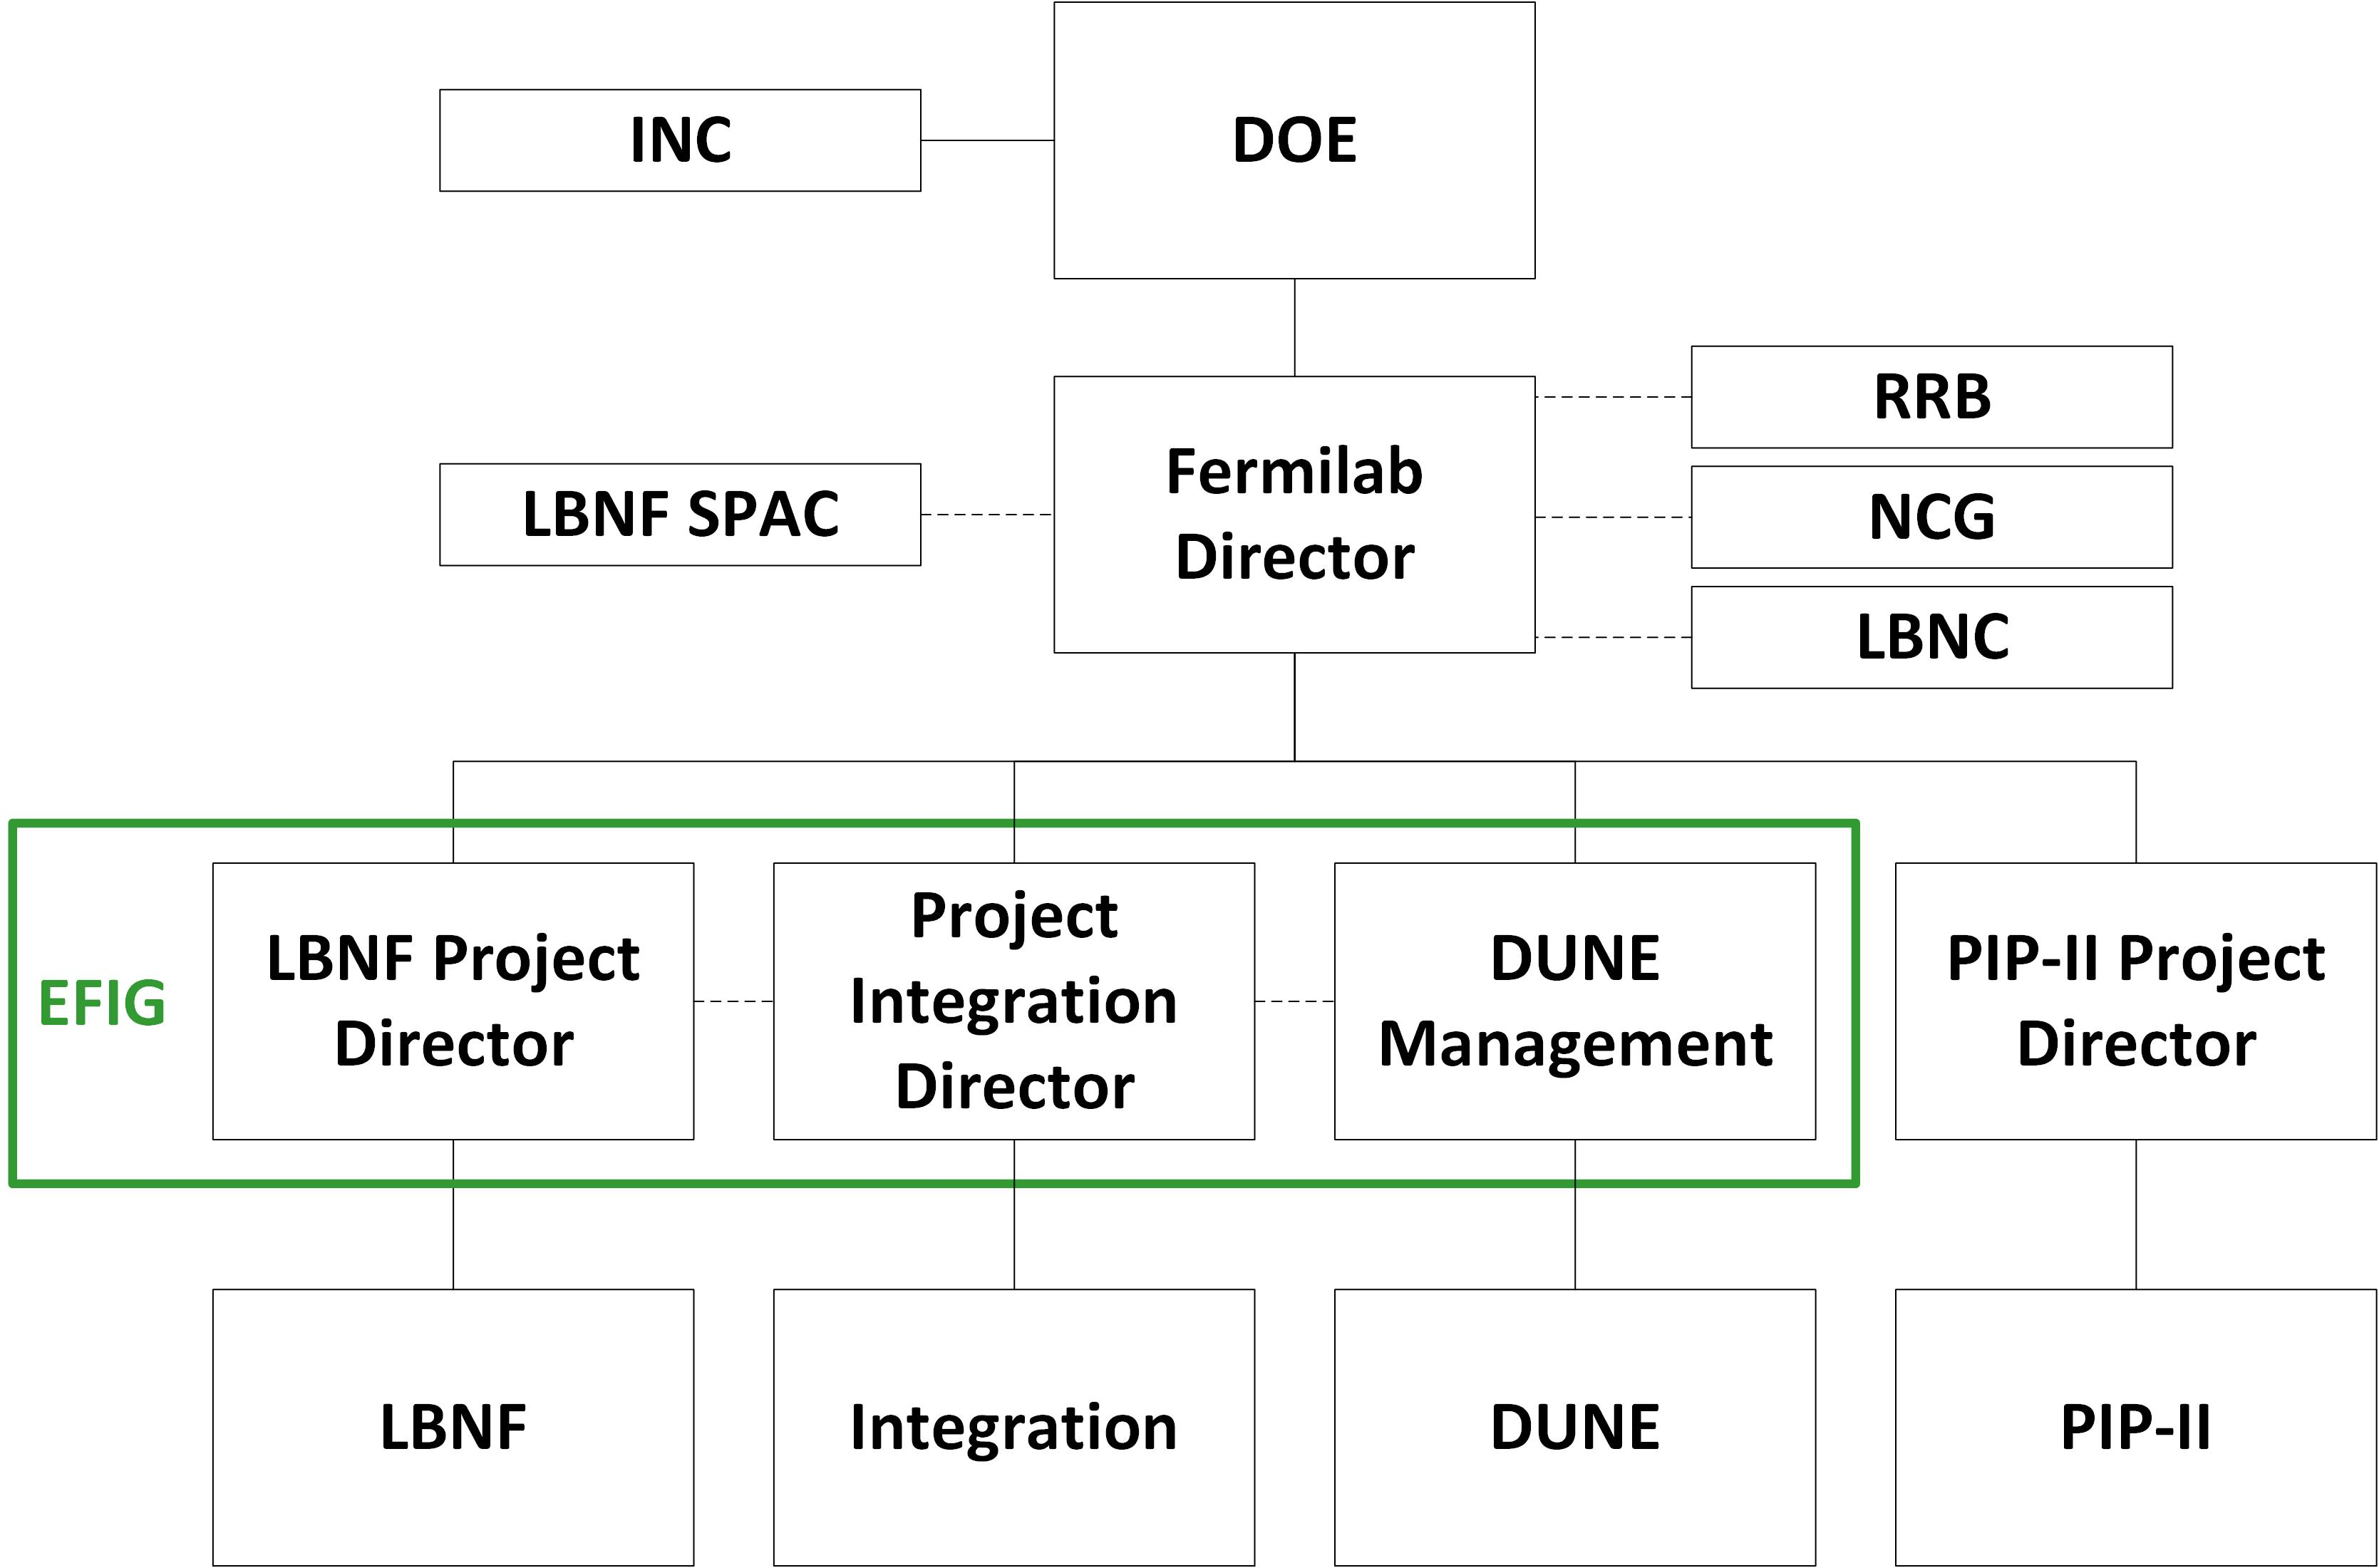
\includegraphics[width=0.67\textwidth]{lbnf_dune_org.jpg}  
\end{dunefigure}

\fixme{we have not addressed SPAC in the diagram}

%%%%%%%%%%%%%%%%%%%%%%%%%%%%%%%%%%%%%%%%%%%%%
\section{DUNE Collaboration Organization and Management}
\label{sec:exec:collab:org}

The \dword{dune} collaboration organizes and manages \dword{dune} in its entirety.  Stakeholders include all collaborating institutions, %including \dword{cern}, 
the funding agencies participating in \dword{dune}, and \dword{fnal} as the host laboratory.  All collaborating institutions have a representative on the \dword{dune} institutional board (IB), which is responsible for establishing the governance rules of the collaboration and regulating governance-related issues. The collaboration is responsible for the design, construction, installation, commissioning, and operation of the detectors and prototypes used to pursue the scientific program. The \dword{dune} \dword{exb}, described below, is the primary management body of the collaboration and approves all significant strategic and technical decisions.

The top-level \dword{dune} collaboration management team consists of two elected co-spokespersons, a \dword{tcoord}, and a \dword{rcoord}. The \dword{tcoord} and \dword{rcoord} are selected jointly by the co-spokespersons and the \dword{fnal} director. The management team is responsible for the day-to-day management of the collaboration and for developing the overall collaboration strategy, which is presented for approval to the \dword{exb}. The \dword{exb} %is the primary collaboration decision-making body and 
comprises the leaders of the main collaboration activities and currently includes %. The composition of the Executive Board, currently including 
the top-level management team, institutional board chair, physics coordinator, beam interface coordinator, computing coordinator, \dword{nd} coordinator, and leaders of the \dword{fd} consortia, described below. It is responsible for  ensuring that all stakeholders in the collaboration have a voice in making decisions (see Figure~\ref{fig:eb}). 
Once the \dword{dune} \dword{fd}  \dword{tdr} is accepted, consortium leaders and coordinators of other major collaboration activities will become elected positions.

\begin{dunefigure}[DUNE executive board]	
{fig:eb}{\dword{dune}{} Executive Board.}
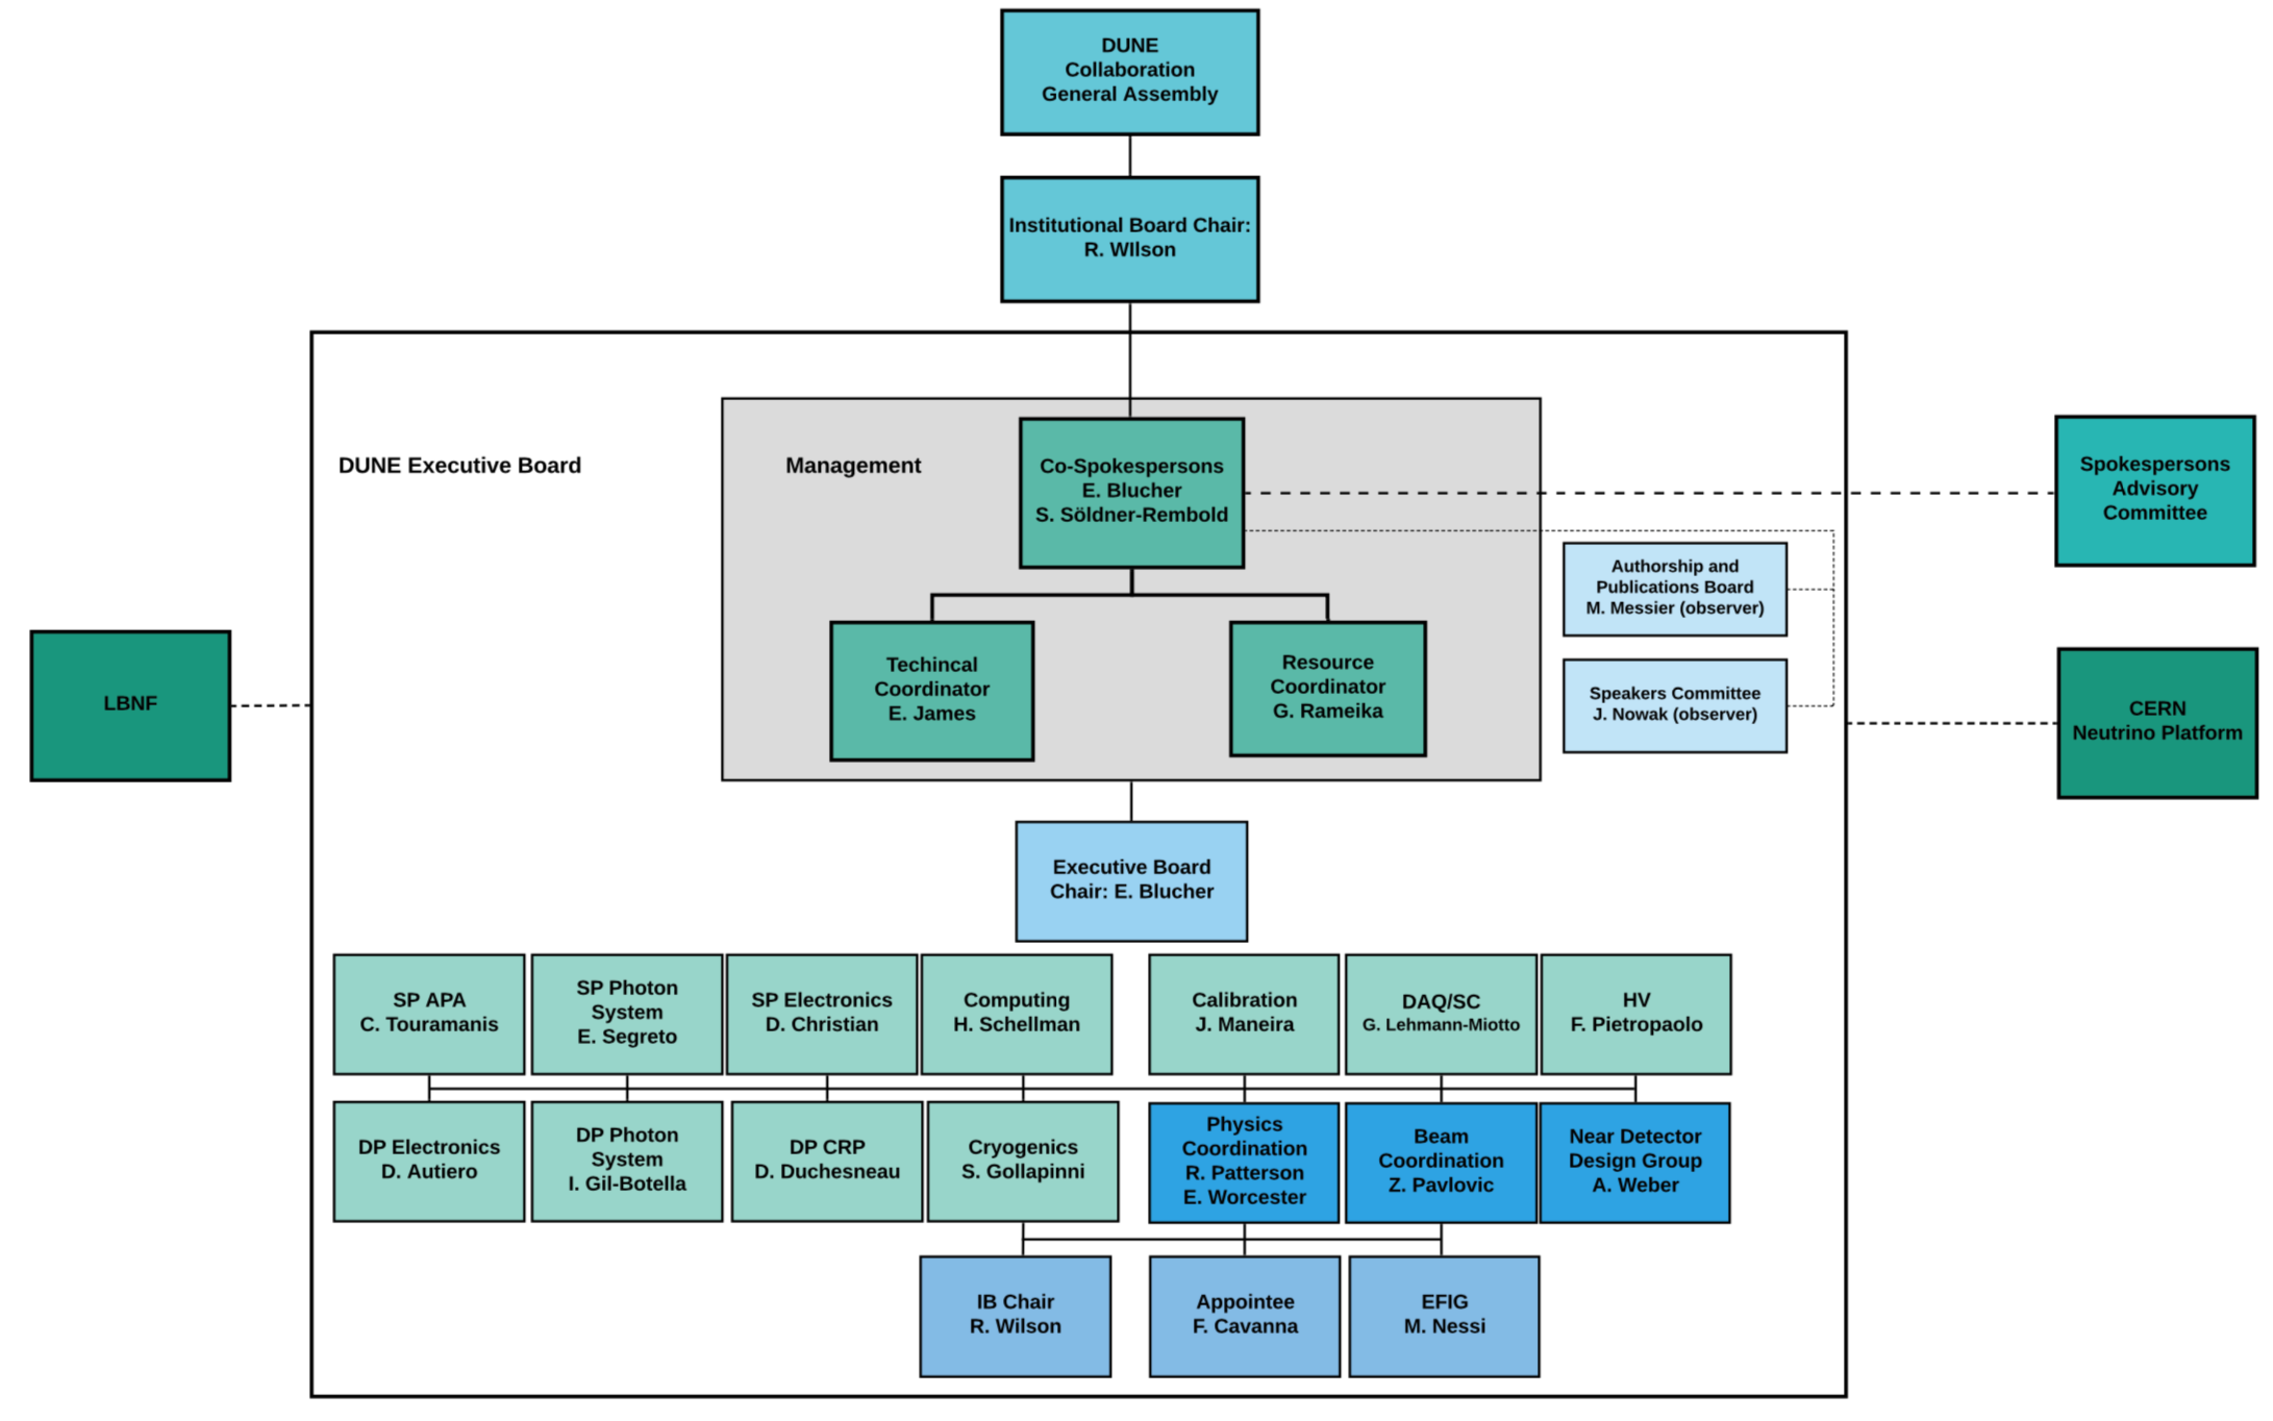
\includegraphics[width=1.3\textwidth, angle=90]{eb.pdf}
\end{dunefigure}

To carry out design and construction work for the \dword{dune} \dword{fd}, \dword{dune} has  formed consortia of institutions, each of which is responsible for an individual detector subsystem. A similar structure will be formed for the \dword{nd} once the final detector concept is selected. The \dword{fd} currently includes eleven consortia, including three specific to \dword{sp}, three specific to \dword{dp}, and five common to both technologies:
\begin{itemize}
\item (\single) \dfirsts{apa}, %Anode Plane Assemblies% (C. Touramanis, UK)
\item (\single) \dfirst{tpc} electronics, %\dword{ce}, % (D. Christian, US)
\item (\single) \dfirst{pds}, %Photon Detection System% (E. Segreto, Brazil)
\item (\dual) \dfirsts{crp}, %Charge Readout Planes% (D. Duchesneau, France)
\item (\dual) \dfirst{tpc} electronics, %(D. Autiero, France)
\item (\dual) \dfirst{pds}, %(PDS), %Photon Detection System %(I. Gil-Botella, Spain)
\item (common) \dword{hvs}, %system, %(F. Pietropaolo, CERN)
\item (common) \dword{daq},  %system, %DAQ System %(D. Newbold, UK)
\item (common) \dword{cisc}, %system, %Slow Controls and Instrumentation. %(S. Gollapinni, US)
\item (common) calibration,  and %system, and
\item (common) computing.
\end{itemize} 
 Each consortium has an overall leader, a technical lead, and a consortium board with representatives from each participating institution. The consortia have full responsibility for their subsystems and for developing a \dword{wbs}, and are expected to understand and document all interfaces with other systems, prepare final technical designs, and draft their own sections of the \dword{tdr}. Following approval of the  \dword{tdr}, they will be responsible for constructing their respective detector subsystems. %In addition to a variety of other tasks, the consortia are responsible for writing their respective sections of the technical proposal and the TDR.

Chapter~\ref{ch:exec-tc} of this volume %provides a more complete introduction to 
introduces the \dword{dune} management and organization specifically as it relates to the \dword{fd}; and Volume~\volnumbertc{}, \voltitletc{}, of the \dword{tdr} provides more detail.

%%%%%%%%%%%%%%%%%%%%%%%%%%%%%%%%%%%%%%%%%%%%%%%%%%%%%%%%%%%%%%% 
\section{Milestones for the First Two Far Detector Modules} 

The plan for construction and commissioning of the first two \dword{fd} modules includes a set of key milestones and dates % and can be found in the \dword{tdr}.  The dates 
that will be finalized once the international project baseline is established.  Table~\ref{tab:es-key-dates} shows the key dates and milestones (colored rows) and indicates how the detector consortia will add subsystem-specific milestones based on these dates (no background color).
 
\begin{dunetable}
[Key milestones and dates]
{p{0.65\textwidth}p{0.25\textwidth}}
{tab:es-key-dates}
{High level construction schedule milestones leading to commissioning the first two  \dword{fd}{} modules. Key \dword{dune}{} dates and milestones, found in this \dword{tdr}{}, are shown in orange.  Dates will be final following establishment of the international project baseline.}   
Milestone & Date   \\ \toprowrule
Technology Decision  &   April 2020   \\ \colhline
Final Design Reviews &   2020   \\ \colhline
\rowcolor{dunepeach} Start of \dshort{pdsp}-II installation& \startpduneiispinstall      \\ \colhline
Production Readiness Reviews  &  2022    \\ \colhline
\rowcolor{dunepeach} Start of \dshort{pddp}-II installation& \startpduneiidpinstall      \\ \colhline
South Dakota Logistics Warehouse available& \sdlwavailable      \\ \colhline
\rowcolor{dunepeach}Beneficial occupancy of cavern 1 and central utility cavern (\dword{cuc})& \cucbenocc      \\ \colhline
\dshort{cuc} data acquisition (DAQ) room accessible& \accesscuccountrm      \\ \colhline
Top of \dshort{detmodule} \#1 cryostat accessible& \accesstopfirstcryo      \\ \colhline
\rowcolor{dunepeach}Start of \dshort{detmodule} \#1 \dshort{tpc} installation& \startfirsttpcinstall      \\ \colhline
Top of \dshort{detmodule} \#2 cryostat accessible& \accesstopsecondcryo      \\ \colhline
End of \dshort{detmodule} \#1 \dshort{tpc} installation& \firsttpcinstallend      \\ \colhline
 \rowcolor{dunepeach}Start of \dshort{detmodule} \#2 \dshort{tpc} installation& \startsecondtpcinstall      \\ \colhline
End of \dshort{detmodule} \#2 \dshort{tpc} installation& \secondtpcinstallend      \\  \colhline
\rowcolor{dunepeach} \dshort{detmodule} \#1 operations & July 2026  \\  
\end{dunetable}


The schedule for the design and construction of \dword{lbnf} and \dword{dune} has two critical parallel paths: one for the far site (South Dakota) %(\surf) and %one 
and another for the %Near Site scope at 
near site (Illinois). %(\dword{fnal}). 
The schedule for initial work is driven by the design and construction of the \dword{cf} (conventional facilities).

During the initial phase of the project, the far site \dword{cf} has been given priority. %comes first. 
Early far site preparation should be complete 
before excavation begins, once %Ross Shaft rehabilitation work is complete. 
rehabilitation work on the Ross Shaft, the shaft providing access to the \dword{dune} underground area, is complete.
\fixme{I think this is done} As each detector 
 cavern is excavated and sufficient utilities are installed, the cryostat construction and cryogenics system installation begins, followed by detector installation, filling with \dword{lar}, and commissioning. 
The first \dword{detmodule} is scheduled to be operational in 2026.

U.S. \dword{doe} project management requires approval at \dword{doecd} milestones before allowing the \dword{lbnf}/\dword{dune} project to move on to the next step. 
CD-1R was granted in 2015, and CD-3A for \dword{lbnf} far site construction was granted in 2016. 
In 2020, \dword{dune} and \dword{lbnf} will seek CD-2/3b and 
%in fall 2020, \dword{dune} and \dword{lbnf} will seek 
 CD-2/3 for the near site. 
The project will conclude with CD-4 approval to start operations.

\begin{comment}
%%%%%%%%%%%%%%%%%%%%%%%%%%%%%%%%%%%%%%%%%%%%%%%%%%%%%%%%%%%%%%%
\section{About the DUNE Far Detector TDR} 
\fixme{needed?}

This multi-volume document constitutes the \dword{tdr} for the \dword{dune} \dword{fd} and covers the technology choices for the first three far detector modules. The \dword{dune} \dword{fd} designs have been prototyped with the two \dword{protodune} detectors at \dword{cern}, and these designs, while largely complete, are undergoing adjustments following lessons learned. Producing detector components is being planned. The \dword{dune} \dword{tdr}, therefore, presents a final technical design for most elements, as well as the few remaining alternative or enhanced designs under consideration. The \dword{tdr} represents the state of the design for these first three \dword{dune} \dword{fd} modules. The fourth module could implement a new \dword{lartpc} configuration, taking into account  potential advances in technology to enhance sensitivity for physics discoveries. 

The \dword{tdr} additionally details the physics goals of the \dword{dune} collaboration and describes the detector designs that will achieve these goals. The \dword{tdr} includes dedicated volumes on the \dword{dune} physics program, the \dword{dune} \dwords{fd}, and the \dword{dune} \dword{tc} organization. In addition to providing overviews of the other volumes, this executive summary volume also includes dedicated chapters on the \dword{nd} and on computing, which will be the subject of future reports. The \dword{nd} \dword{tdr} is planned for 2020, and the computing Conceptual Design Report will be provided on a similar timescale.



%%%%%%%%%%%%%%%%%%%%%%%%%%%%%%%%%%%%%%%%%%%%%%%%%%%%%%%%%%%%%%
\section{Organization of the DUNE Technical Design Report}

\fixme{With the preface, this section probably isn't needed anymore. Anne}

The \dword{dune} FD \dword{tdr} describes the experiment's proposed physics program, the 
technical designs of the two \dword{fd} \dword{lartpc} technologies, and the technical coordination required to construct and commission the first far \dwords{detmodule}.
The \dword{tdr} will justifies the technical choices that flow down from the high-level physics goals through requirements at all levels of the project. These design choices will enable the \dword{dune} experiment to make the ground-breaking discoveries that will help answer 
fundamental physics questions. 

To accomplish this, the \dword{dune} \dword{fd} \dword{tdr} is divided into five volumes:

\begin{itemize}
\item Volume~\volnumberexec{} provides the executive summary of the overall experimental program. It includes a brief description of the \dword{dune} science program, the \dword{dune} detectors, and technical coordination, which are subjects of the remaining volumes in the \dword{tdr}. This volume also includes a description of two systems not yet at the technical design stage: the \dword{dune} \dword{nd} and \dword{dune} computing, such that one can get a full picture of overall plans for DUNE.
\item Volume~\volnumberphysics{} outlines the scientific objectives and describes the physics studies that the \dword{dune} collaboration will undertake and the methods for meeting those objectives.
\item Volume~\volnumbertc{} describes the organizational structures,  methodologies, procedures, requirements, risks, and other technical  coordination aspects of constructing the first two \dword{fd} modules in South Dakota.
\item Volume~\volnumbersp{} describes the \dword{sp} \dword{fd} technology, subsystems, and components that the first (and any subsequent) \dword{sp} \dwords{detmodule} will comprise, as well as the installation plan for the first \dword{fd} module, which will be of this type. 
\item Volume~\volnumberdp{} describes the \dword{dp} \dword{fd} technology, the subsystems, and components that  the first (and any subsequent) \dword{dp} \dwords{detmodule} will comprise, as well as the installation plan for the first \dword{dp} module. 
\end{itemize}

\end{comment}
